% Options for packages loaded elsewhere
\PassOptionsToPackage{unicode}{hyperref}
\PassOptionsToPackage{hyphens}{url}
%
\documentclass[
  man]{apa7}
\usepackage{amsmath,amssymb}
\usepackage{iftex}
\ifPDFTeX
  \usepackage[T1]{fontenc}
  \usepackage[utf8]{inputenc}
  \usepackage{textcomp} % provide euro and other symbols
\else % if luatex or xetex
  \usepackage{unicode-math} % this also loads fontspec
  \defaultfontfeatures{Scale=MatchLowercase}
  \defaultfontfeatures[\rmfamily]{Ligatures=TeX,Scale=1}
\fi
\usepackage{lmodern}
\ifPDFTeX\else
  % xetex/luatex font selection
\fi
% Use upquote if available, for straight quotes in verbatim environments
\IfFileExists{upquote.sty}{\usepackage{upquote}}{}
\IfFileExists{microtype.sty}{% use microtype if available
  \usepackage[]{microtype}
  \UseMicrotypeSet[protrusion]{basicmath} % disable protrusion for tt fonts
}{}
\makeatletter
\@ifundefined{KOMAClassName}{% if non-KOMA class
  \IfFileExists{parskip.sty}{%
    \usepackage{parskip}
  }{% else
    \setlength{\parindent}{0pt}
    \setlength{\parskip}{6pt plus 2pt minus 1pt}}
}{% if KOMA class
  \KOMAoptions{parskip=half}}
\makeatother
\usepackage{xcolor}
\usepackage{graphicx}
\makeatletter
\def\maxwidth{\ifdim\Gin@nat@width>\linewidth\linewidth\else\Gin@nat@width\fi}
\def\maxheight{\ifdim\Gin@nat@height>\textheight\textheight\else\Gin@nat@height\fi}
\makeatother
% Scale images if necessary, so that they will not overflow the page
% margins by default, and it is still possible to overwrite the defaults
% using explicit options in \includegraphics[width, height, ...]{}
\setkeys{Gin}{width=\maxwidth,height=\maxheight,keepaspectratio}
% Set default figure placement to htbp
\makeatletter
\def\fps@figure{htbp}
\makeatother
\setlength{\emergencystretch}{3em} % prevent overfull lines
\providecommand{\tightlist}{%
  \setlength{\itemsep}{0pt}\setlength{\parskip}{0pt}}
\setcounter{secnumdepth}{-\maxdimen} % remove section numbering
% Make \paragraph and \subparagraph free-standing
\makeatletter
\ifx\paragraph\undefined\else
  \let\oldparagraph\paragraph
  \renewcommand{\paragraph}{
    \@ifstar
      \xxxParagraphStar
      \xxxParagraphNoStar
  }
  \newcommand{\xxxParagraphStar}[1]{\oldparagraph*{#1}\mbox{}}
  \newcommand{\xxxParagraphNoStar}[1]{\oldparagraph{#1}\mbox{}}
\fi
\ifx\subparagraph\undefined\else
  \let\oldsubparagraph\subparagraph
  \renewcommand{\subparagraph}{
    \@ifstar
      \xxxSubParagraphStar
      \xxxSubParagraphNoStar
  }
  \newcommand{\xxxSubParagraphStar}[1]{\oldsubparagraph*{#1}\mbox{}}
  \newcommand{\xxxSubParagraphNoStar}[1]{\oldsubparagraph{#1}\mbox{}}
\fi
\makeatother
% definitions for citeproc citations
\NewDocumentCommand\citeproctext{}{}
\NewDocumentCommand\citeproc{mm}{%
  \begingroup\def\citeproctext{#2}\cite{#1}\endgroup}
\makeatletter
 % allow citations to break across lines
 \let\@cite@ofmt\@firstofone
 % avoid brackets around text for \cite:
 \def\@biblabel#1{}
 \def\@cite#1#2{{#1\if@tempswa , #2\fi}}
\makeatother
\newlength{\cslhangindent}
\setlength{\cslhangindent}{1.5em}
\newlength{\csllabelwidth}
\setlength{\csllabelwidth}{3em}
\newenvironment{CSLReferences}[2] % #1 hanging-indent, #2 entry-spacing
 {\begin{list}{}{%
  \setlength{\itemindent}{0pt}
  \setlength{\leftmargin}{0pt}
  \setlength{\parsep}{0pt}
  % turn on hanging indent if param 1 is 1
  \ifodd #1
   \setlength{\leftmargin}{\cslhangindent}
   \setlength{\itemindent}{-1\cslhangindent}
  \fi
  % set entry spacing
  \setlength{\itemsep}{#2\baselineskip}}}
 {\end{list}}
\usepackage{calc}
\newcommand{\CSLBlock}[1]{\hfill\break\parbox[t]{\linewidth}{\strut\ignorespaces#1\strut}}
\newcommand{\CSLLeftMargin}[1]{\parbox[t]{\csllabelwidth}{\strut#1\strut}}
\newcommand{\CSLRightInline}[1]{\parbox[t]{\linewidth - \csllabelwidth}{\strut#1\strut}}
\newcommand{\CSLIndent}[1]{\hspace{\cslhangindent}#1}
\ifLuaTeX
\usepackage[bidi=basic]{babel}
\else
\usepackage[bidi=default]{babel}
\fi
\babelprovide[main,import]{english}
% get rid of language-specific shorthands (see #6817):
\let\LanguageShortHands\languageshorthands
\def\languageshorthands#1{}
% Manuscript styling
\usepackage{upgreek}
\captionsetup{font=singlespacing,justification=justified}

% Table formatting
\usepackage{longtable}
\usepackage{lscape}
% \usepackage[counterclockwise]{rotating}   % Landscape page setup for large tables
\usepackage{multirow}		% Table styling
\usepackage{tabularx}		% Control Column width
\usepackage[flushleft]{threeparttable}	% Allows for three part tables with a specified notes section
\usepackage{threeparttablex}            % Lets threeparttable work with longtable

% Create new environments so endfloat can handle them
% \newenvironment{ltable}
%   {\begin{landscape}\centering\begin{threeparttable}}
%   {\end{threeparttable}\end{landscape}}
\newenvironment{lltable}{\begin{landscape}\centering\begin{ThreePartTable}}{\end{ThreePartTable}\end{landscape}}

% Enables adjusting longtable caption width to table width
% Solution found at http://golatex.de/longtable-mit-caption-so-breit-wie-die-tabelle-t15767.html
\makeatletter
\newcommand\LastLTentrywidth{1em}
\newlength\longtablewidth
\setlength{\longtablewidth}{1in}
\newcommand{\getlongtablewidth}{\begingroup \ifcsname LT@\roman{LT@tables}\endcsname \global\longtablewidth=0pt \renewcommand{\LT@entry}[2]{\global\advance\longtablewidth by ##2\relax\gdef\LastLTentrywidth{##2}}\@nameuse{LT@\roman{LT@tables}} \fi \endgroup}

% \setlength{\parindent}{0.5in}
% \setlength{\parskip}{0pt plus 0pt minus 0pt}

% Overwrite redefinition of paragraph and subparagraph by the default LaTeX template
% See https://github.com/crsh/papaja/issues/292
\makeatletter
\renewcommand{\paragraph}{\@startsection{paragraph}{4}{\parindent}%
  {0\baselineskip \@plus 0.2ex \@minus 0.2ex}%
  {-1em}%
  {\normalfont\normalsize\bfseries\itshape\typesectitle}}

\renewcommand{\subparagraph}[1]{\@startsection{subparagraph}{5}{1em}%
  {0\baselineskip \@plus 0.2ex \@minus 0.2ex}%
  {-\z@\relax}%
  {\normalfont\normalsize\itshape\hspace{\parindent}{#1}\textit{\addperi}}{\relax}}
\makeatother

\makeatletter
\usepackage{etoolbox}
\patchcmd{\maketitle}
  {\section{\normalfont\normalsize\abstractname}}
  {\section*{\normalfont\normalsize\abstractname}}
  {}{\typeout{Failed to patch abstract.}}
\patchcmd{\maketitle}
  {\section{\protect\normalfont{\@title}}}
  {\section*{\protect\normalfont{\@title}}}
  {}{\typeout{Failed to patch title.}}
\makeatother

\usepackage{xpatch}
\makeatletter
\xapptocmd\appendix
  {\xapptocmd\section
    {\addcontentsline{toc}{section}{\appendixname\ifoneappendix\else~\theappendix\fi\\: #1}}
    {}{\InnerPatchFailed}%
  }
{}{\PatchFailed}
\keywords{Employee turnover, machine learning\newline\indent Word count: X}
\DeclareDelayedFloatFlavor{ThreePartTable}{table}
\DeclareDelayedFloatFlavor{lltable}{table}
\DeclareDelayedFloatFlavor*{longtable}{table}
\makeatletter
\renewcommand{\efloat@iwrite}[1]{\immediate\expandafter\protected@write\csname efloat@post#1\endcsname{}}
\makeatother
\usepackage{csquotes}
\usepackage[titles]{tocloft}
\cftpagenumbersoff{figure}
\renewcommand{\cftfigpresnum}{\itshape\figurename\enspace}
\renewcommand{\cftfigaftersnum}{.\space}
\setlength{\cftfigindent}{0pt}
\setlength{\cftafterloftitleskip}{0pt}
\settowidth{\cftfignumwidth}{Figure 10.\qquad}
\cftpagenumbersoff{table}
\renewcommand{\cfttabpresnum}{\itshape\tablename\enspace}
\renewcommand{\cfttabaftersnum}{.\space}
\setlength{\cfttabindent}{0pt}
\setlength{\cftafterloftitleskip}{0pt}
\settowidth{\cfttabnumwidth}{Table 10.\qquad}
\setlength{\parskip}{0pt}
\newcommand{\bcenter}{\begin{center}}
\newcommand{\ecenter}{\end{center}}
\raggedbottom
\usepackage{wrapfig}
\usepackage{multicol}
\setlength{\columnsep}{5cm}
\usepackage{fancyhdr}
\usepackage{setspace}
\pagestyle{fancy}
\ifLuaTeX
  \usepackage{selnolig}  % disable illegal ligatures
\fi
\usepackage{bookmark}
\IfFileExists{xurl.sty}{\usepackage{xurl}}{} % add URL line breaks if available
\urlstyle{same}
\hypersetup{
  pdfauthor={Diego Figueiras1},
  pdflang={en-EN},
  pdfkeywords={Employee turnover, machine learning},
  hidelinks,
  pdfcreator={LaTeX via pandoc}}

\title{TITLE}
\author{Diego Figueiras\textsuperscript{1}}
\date{}


\shorttitle{Influence of Parsimony}

\authornote{

Correspondence concerning this article should be addressed to Diego Figueiras, Dickson Hall 226. E-mail: \href{mailto:figueirasd1@montclair.edu}{\nolinkurl{figueirasd1@montclair.edu}}

}

\affiliation{\vspace{0.5cm}\textsuperscript{1} Montclai State University}

\begin{document}
\maketitle

\thispagestyle{empty}
\newpage

\renewcommand{\headrulewidth}{0pt}
\renewcommand{\footrulewidth}{0pt}
\pagenumbering{gobble}
\phantom{i'm a ghost}
\vskip 1.0in
\begin{center}

\textbf{Influence of Parsimony and Work-related Psychological Constructs in Predicting Turnover Intention when Using Machine Learning VS Regression}

\vskip 0.8in

A DISSERTATION

\vskip 0.8in

Submitted to the Faculty of

Montclair State University in partial fulfillment

of the requirements

for the degree of Doctor of Philosophy

\vskip 0.4in

by

Diego Figueiras

Montclair State University

Montclair, NJ

May 2024

\end{center}

\vskip 1.0in

Dissertation Chair: Dr.~Michael Bixter

\newpage

\section{}
\pagenumbering{roman}
\fancyhead[LO, LE]{INFLUENCE OF PARSIMONY}
\cfoot{}
\rhead{\thepage}

\renewcommand{\headrulewidth}{0pt}
\renewcommand{\footrulewidth}{0pt}

\onehalfspacing

\begin{center}

MONTCLAIR STATE UNIVERSITY

THE GRADUATE SCHOOL

DISSERTATION APPROVAL

\vskip 0.2in

We hereby approve the Dissertation

\vskip 0.2in

\textbf{Influence of Parsimony and Work-related Psychological Constructs in Predicting Turnover Intention when Using Machine Learning VS Linear Regression}

of

Diego Figueiras

Candidate for the Degree:

Doctor of Philosophy

\end{center}

\begin{multicols}{2}  


\noindent{Graduate Programs:}
\newline
Counseling

\vskip 0.6in

\noindent{Certified by:}

\vskip 0.6in  

\linespread{1.0}\selectfont
\noindent\rule{6cm}{0.2mm}
\newline
Dr. Kenneth Sumner 
\newline
Associate Provost for Academic Affairs and
\newline
Acting Dean of the Graduate School

\vskip 0.3in

\noindent\rule{6cm}{0.2mm}
\newline
Date

\columnbreak

\noindent{Dissertation Committee:}

\vskip 0.6in

\noindent\rule{6cm}{0.2mm}
\newline
Dr. Michael Bixter
\newline
Dissertation Chair

\vskip 0.6in

\noindent\rule{6cm}{0.2mm}
\newline
Dr. Kevin Askew

\vskip 0.6in

\noindent\rule{6cm}{0.2mm}
\newline
Dr. John T. Kulas


\end{multicols}

\newpage
\fancyhead[LO, LE]{INFLUENCE OF PARSIMONY}
\renewcommand{\headrulewidth}{0pt}
\renewcommand{\footrulewidth}{0pt}

\begin{center}

\phantom{i'm a ghost}

\vskip 1.6in

\href{mailto:Copyright@2024}{\nolinkurl{Copyright@2024}} by Diego Figueiras. All rights reserved.

\end{center}

\newpage
\fancyhead[LO, LE]{INFLUENCE OF PARSIMONY}
\renewcommand{\headrulewidth}{0pt}
\renewcommand{\footrulewidth}{0pt}

\begin{center}

\textbf{Abstract}

\end{center}

This dissertation explores the ongoing debate between traditional statistical regression models and machine learning (ML) algorithms in predictive modeling, focusing on the impact of sample size and the number of variables. Study 1 investigates the relationship between sample size and predictive accuracy, proposing hypotheses regarding the advantages of ML over regression as sample size increases. Additionally, the study examines the influence of the number of variables on predictive accuracy, emphasizing the trade-off between ML and regression models. Using data from the Federal Employee Viewpoint Survey, the research aims to contribute insights into the conditions favoring each modeling approach. Study 2 shifts the focus to incremental validity, exploring whether work-related psychological constructs enhance ML models' predictive accuracy in turnover intention compared to biodata alone. The proposed hypotheses suggest that incorporating psychological constructs will improve predictive accuracy, addressing the ``garbage in garbage out'' concern prevalent in ML applications. The methods involve diverse datasets, including responses from federal employees and an online survey through Amazon's MTurk, with machine learning algorithms such as Gradient Boosting Trees, Random Forest, Neural Networks, and Support Vector Machines being compared to linear and logistic regressions. The dissertation seeks to advance understanding in the field, offering practical insights for researchers and practitioners navigating the dynamic landscape of predictive modeling.

\newpage
\fancyhead[LO, LE]{INFLUENCE OF PARSIMONY}
\pagenumbering{arabic}
\renewcommand{\headrulewidth}{0pt}
\renewcommand{\footrulewidth}{0pt}

\tableofcontents

\section{Chapter 1 (Heading 1)}
\newpage

\section{Introduction}\label{introduction}

Employee turnover is a critical concern for organizations, as it impacts productivity, performance, and overall organizational effectiveness (Griffeth et al., 2000).
Accurate prediction of turnover is crucial for proactive human resource management and the implementation of effective retention strategies (T. R. Mitchell et al., 2001; Mobley et al., 1979).
In recent years, the application of predictive modeling techniques has gained prominence in addressing this challenge.
The debate arises as to whether regression-based models or machine learning models are more effective in predicting turnover, particularly when working with small sample sizes.

The high amount of computer power in the cloud environment nowadays and the developments in the field of machine learning are providing easy access to high-performance services.
Machine learning-supported tools are enabling companies to analyze and evaluate information in a quick and effective way (Tambe et al., 2019).
We see this in the form of applications, software, and solutions that are common in business or that automate the different decision-making processes, such as programs that create and post job descriptions, application tracking systems that identify key words to place candidates in the right openings, tools for scheduling interviews with your online calendar, chatbots for screening, etc (Rąb-Kettler \& Lehnervp, 2019).
Human resources practices are not being oblivious to these developments.
Experts in these practices are realizing the advantages of data-driven decision making (Fallucchi et al., 2020).
Large amounts of human resources data can be analyzed in a short time and empirical inferences can be made, enabling experts to better understand employees and help anticipate issues and patterns (Macijauskien \& Stankevi, 2021).
Being able to predict the best suited personnel for positioning or that will turn over is of particular interest to human resource departments and companies in general.
Making the wrong decision when giving a promotion or demotion can cause waste of time and energy, as well as compromise the perceived organizational justice and support, resulting in more turnover.
This is why personnel placement processes are some of the most pivotal in human resources (Macijauskien \& Stankevi, 2021).

When making decisions for placement using traditional regression-based methods, there is a high probability of this being affected by subjective factors that can cause biased choices from time to time (Fallucchi et al., 2020).
With machine learning, on the other hand, these decisions are based on a bit more objective foundation than most other recommended methods, since it is based solely on the patterns the algorithm finds on the data (though there can still be bias in the development or implementation of particular algorithms, this is minimized in comparison with traditional methods) (Raji \& Buolamwini, 2019; Zou \& Schiebinger, 2018).
Not only this, but the decisions made in the personnel placement process can be explained to the candidates with their reasons, providing them with confidence in the results and diminishing the chances of low perceived organizational justice/support and high turnover.

The aim of this dissertation is to investigate and compare the predictive capabilities of regression-based models and machine learning models in the context of turnover prediction, focusing specifically on sample sizes and number of variables.
By examining the strengths and limitations of these modeling approaches, this study seeks to shed light on which combination of methods and data characteristics offers greater accuracy and reliability in predicting turnover within resource-constrained environments. Hopefully, this will inform practices in the decision-making process when using these algorithms.

Regression-based models, including linear regression, logistic regression, and Cox proportional hazards regression, have long been established as prominent tools in predictive modeling (Cox, 1972; Hosmer Jr et al., 2013).
These models are characterized by their simplicity, interpretability, and assumption of linearity between predictors and the outcome variable (or the logit of the outcome variable in the case of binary logistic regression).
The straightforward nature of regression-based models allows for the identification of significant predictors and estimation of their individual effects, facilitating an understanding of the underlying mechanisms driving turnover (Hom et al., 2009; Meyer et al., 2004).

Contrarily, machine learning models have garnered significant attention due to their ability to handle complex relationships and patterns in large datasets (Breiman, 2001a; Hastie et al., 2009).
Algorithms such as random forests, support vector machines, and artificial neural networks offer the potential to capture non-linear and interactive effects without having to specify a theoretical model, making them valuable tools in predictive modeling (Kermany et al., 2018; Niculescu-Mizil \& Caruana, 2005).
Machine learning models have been increasingly applied to turnover prediction, displaying promising results in various studies (Biswas et al., 2020).

While the application of machine learning models has gained momentum, their performance in the context of small sample sizes remains an open question.
The literature suggests that machine learning models may face challenges, such as overfitting, when trained on limited data (Varoquaux, 2018; Xu et al., 2020).
Consequently, the predictive performance of these models might be compromised when sample sizes are below a certain threshold.
Thus, it becomes imperative to evaluate whether regression-based models, with their simplicity and interpretability, outperform machine learning models when the sample size is small enough.

Additionally, the performance of machine learning models may be affected when the number of independent variables is small.
In such scenarios, these models may face challenges such as overfitting or difficulty in identifying meaningful patterns (Guyon \& Elisseeff, 2003; Varoquaux, 2018).
On the other hand, regression-based models may offer advantages in situations where the number of independent variables is limited, as they are less prone to overfitting and can provide transparent insights into the relationships between predictors and turnover (Hosmer Jr et al., 2013).

Traditional variables in the demographic and biodata domain, such as age, gender, and education, have been commonly used in turnover prediction models (Hom et al., 2012; Meyer et al., 2004).
However, the utilization of antecedent variables typically studied in the field of I-O psychology, such as job satisfaction, organizational commitment, and conscientiousness, may provide deeper insights into the underlying factors contributing to turnover (Hom et al., 2012; Lee et al., 2021).

The application of work-related psychological antecedent variables in machine learning-based models holds promise for improving turnover prediction accuracy.
These variables capture psychological and organizational aspects that directly impact employees' turnover intentions and behaviors (Lee et al., 2021; Meyer et al., 2004).
By considering these variables in predictive models, organizations can gain a more comprehensive understanding of the complex dynamics that drive turnover and develop targeted interventions to mitigate it (Griffeth et al., 2000; Hom et al., 2012).

Contrarily, models relying solely on demographics and biodata may overlook critical factors contributing to turnover.
While these variables provide basic demographic information, they may lack the depth and specificity necessary to capture the nuances and complexities of turnover behavior (Hom et al., 2012).
Incorporating work-related psychological antecedent variables can offer a more nuanced and accurate prediction by considering individual attitudes, perceptions, and experiences within the organizational context, as has been demonstrated before (Lee et al., 2021; Meyer et al., 2004).

This second study aims to address this research question by employing survey data.
By leveraging turnover intention data and a restricted set of independent variables, along with relevant predictor variables such as demographics/biodata, job characteristics, employee engagement, and other work-related psychological antecedent variables of turnover, a comparative analysis will be conducted.
The performance of regression-based models and machine learning models will be assessed using various metrics, including accuracy, precision, recall, and the area under the receiver operating characteristic curve (AUC-ROC) (Davis \& Goadrich, 2006).

The findings from this research will contribute to the existing literature on turnover prediction and provide valuable insights for practitioners and researchers alike.
Understanding the relative performance of regression-based models and machine learning models when dealing with small sample sizes can guide decision-making regarding the choice of modeling techniques in resource-limited scenarios.
Ultimately, this research aims to enhance our understanding of turnover prediction and inform effective retention strategies to mitigate the negative consequences of employee turnover.

\subsection{What Constitutes Machine Learning}\label{what-constitutes-machine-learning}

The delineation between machine learning (ML) and statistical modeling has been extensively explored in the literature (Breiman, 2001b).
However, the distinction remains ambiguous, as noted by Collins et al. (2014).
Breiman's seminal work on the ``two cultures'' serves as a key reference in this discussion (Breiman, 2001b).
Breiman highlights the contrast between theory-driven models like regression and empirical algorithms such as decision trees, artificial neural networks, support vector machines, and random forests.

\subsection{Theory-based models}\label{theory-based-models}

Theory-based models are models that are based on theory and assumptions, such as traditional linear regression, and benefit from human intervention and subject knowledge for model specification.
The analysis in this approach starts with assuming a stochastic data model for the inside of the black box.
Usually, research that uses this approach starts by assuming that the data are generated by a particular model.
This model is used as a template for statistical analysis.
When faced with an applied problem, researchers that use this approach come up with a data model by looking at the literature developed by previous scholars or by their own theorizing, or some combination of both.
This enables them to develop a reasonably good parametric class of models for a complex mechanism devised by nature, and then parameters are estimated and conclusions are drawn.
However, these conclusions are about the model's mechanism, not about nature's mechanism, and therefore if the model is a poor emulation of nature, the conclusion could be wrong.
Breiman (2001) criticized this approach, pointing out that: ``A few decades ago, the commitment to data models was such that even simple precaution such as residual analysis or goodness-of-fit tests were not used. The belief in the infallibility of the data models was almost religious. It is a strange phenomenon -- once a model is made, then it becomes truth and the conclusions from it are infallible (p.~202).'' He concludes by using the following old saying: ``If all a man has is a hammer, then every problem looks like a nail (p.~202).'' To solve a wide range of problems, such as is the case in the social sciences with the abundance of variables, a larger set of tools is needed.
The rapidly increasing ability of computers to store and manipulate data can provide us with more varied tools.

\subsection{Empirical-based models}\label{empirical-based-models}

In the mid-1980s, with the development of neural networks and decision trees, a new community of researchers appeared focused on predictive accuracy (Cristianini \& Scholkopf, 2002).
They began using these algorithms on working in complex prediction problems where it was obvious that data models were not applicable, such as speech recognition, image recognition, handwriting recognition, times series analysis, or financial market analysis.
The approach is that nature produces data in a black box whose insides are complex and partly unknowable.
The goal is not to explain the patterns in this data, but to predict them based on input; not to focus on data models, but on the characteristics of the algorithms (Breiman, 2001b).
Within psychology, this is the same approach as dustbowl empiricism (Schoenfeldt, 1999).

An effective characterization of machine learning involves its emphasis on models that autonomously glean insights from data (T. M. Mitchell, 1997).
Unlike regression, machine learning exhibits a higher degree of automation in modeling, particularly in handling nonlinear relationships and interaction terms, as exemplified by Boulesteix (Boulesteix \& Schmid, 2014).
Achieving this automation often entails the use of highly adaptable algorithms in machine learning, which may necessitate penalization techniques to prevent overfitting (Deo \& Nallamothu, 2016).
Some scholars depict the relationship between statistical modeling and machine learning as a continuous spectrum (Beam \& Kohane, 2018).
Meanwhile, others categorize any approach deviating from basic regression models as machine learning, encompassing methods like penalized regression (e.g., LASSO, elastic net) or generalized additive models (GAM) (He \& Garcia, 2009).
It is essential to highlight that, according to the ``automatic learning from data'' definition, these methods do not strictly fall under machine learning.
In this study, we refrain from classifying them as such.

\subsection{Common Terms in Machine Learning}\label{common-terms-in-machine-learning}

\begin{itemize}
\item
  Supervised learning: these are algorithms that have a dependent variable they are trying to predict.
  If the dependent variable is discrete, it would be a classifier; if it is continuous, it would be regression-based (Hastie et al., 2009).
  For the purposes of this study we will be focusing on this type of machine learning.
\item
  Unsupervised learning: these are algorithms that do not have a dependent variable that they are trying to predict, but rather look for associations and clusters among the independent variables (Hastie et al., 2009)
\item
  Cross-validation: this is a technique used to assess the performance and generalizability of a predictive model.
  It involves partitioning the dataset into multiple subsets, training the model on some of these subsets, and evaluating its performance on the remaining data.
  This process is repeated multiple times, with different subsets used for training and testing, allowing for a more robust evaluation of the model's effectiveness across various data scenarios (Douglass, 2020).
\item
  Regularization: in machine learning, this is a technique employed to prevent overfitting and enhance the generalization performance of a predictive model by adding a penalty term to the cost function.
  This penalty discourages the model from fitting the training data too closely and helps to control the complexity of the model, preventing it from becoming too intricate and specialized to the training set (Hastie et al., 2009).
\item
  Ensemble: in machine learning, this involves combining predictions from multiple individual models to create a more robust and accurate overall prediction (Dietterich, 2000).
  By leveraging the diversity among the constituent models, ensemble methods aim to improve generalization performance, mitigate overfitting, and enhance predictive accuracy across a variety of scenarios.
\end{itemize}

\subsection{Data Hungriness}\label{data-hungriness}

The concept of data hungriness refers to the sample size needed for a method to generate a prediction model with a good predictive accuracy (Ploeg et al., 2014).
The data hungriness of a predictive modeling technique is defined as the minimum number of events per variable at which the optimism of the generated model is less than 0.01.
Optimism is defined as the difference between error on the sample data and the error when applying the model to another dataset.
Every machine learning model has some amount of error in its predictions.
This error usually comes from two different sources: bias and variance.
Bias is the tendency of the model to underfit, and variance is the tendency to overfit.
The relationship between these two sources of error is known as the bias-variance tradeoff, and developers of machine learning models have to find the balance between the two.

To test if this trade-off has been done in a way that minimizes error, it is a good idea to measure performance using data that the model has never seen before.
The performance of the model on this ``test data'' will be a more accurate predictor of the model's performance in the real world, which is the fundamental basis for cross-validation .
The model's optimism, therefore, is the difference between the training error estimated from the data used to build the model and the test error estimated by applying the model into out-of-sample data.
The sample size needed to minimize this difference is what is referred to as data hungriness.
Machine learning algorithms generally require big sample sizes to minimize this difference (Ploeg et al., 2014).

\subsection{Parsimony}\label{parsimony}

Parsimony is defined as the sample size and number of variables that a dataset must have in order to maximize the predictive accuracy of a model (Sanchez-Pinto, Luo, et al., 2018).
A model is considered parsimonious when it both uses the least amount of variables possible (sparsity) and has good prediction accuracy.
Typically, parsimony is reported as the performance metric of models that are sparse.

\section{Algorithms}\label{algorithms}

In this dissertation, various machine learning algorithms are described and assessed in their ability to predict dependent variables of interest in the field of I/O psychology, specifically turnover intention.
This section provides a general overview of the underlying mechanicsms behind these algorithms.

\subsection{Decision Trees}\label{decision-trees}

Decision trees are a type of supervised machine learning method.
They create classification or regression models following a tree-like structure (Mahesh, 2020).
Each fork is a split in a predictor variables, and in which each end node contains a prediction for the outcome variable (Marsland, 2011).
They are used to explain how the target variable's values can be predicted based on other variables.
Nodes are split into sub-nodes based on a threshold value of a variable (Mahesh, 2020).
Decision trees are capable of handling missing values and mixed features, as well as to select variables automatically.
On the downside, their predictive power is not as high as other algorithms and they are not stable with high model variance and small variations in the data.
This could result in a large effect on the tree structure that is not meaningful.
However, understanding how they operate becomes important in order to understand other algorithms, such as random forest and gradient boosting trees (Alpaydin, 2020; Marsland, 2011).

\subsection{Classification and Regression Trees (CART)}\label{classification-and-regression-trees-cart}

A Classification and Regression Tree is an umbrella term that refers to the use of either classification and/or regression trees (Marsland, 2011).
We already explained classification trees, so lets now explain regression.
Regression trees are a type of decision tree.
They are different from classification trees in that each leaf represents a numeric value, while classification trees have ``true'' or ``false'' in their leaves, or some other discrete category.
The roots and branches of regression trees are typically ranges of the IVs, while the leaves are typically the average value of the DV in those ranges.
The structure of these trees typically starts with the root being the lower threshold of the IVs, and its leaf the average DV at this range.
Then the first branch is the upper threshold, with the leaf being the average DV at that range.
The second branch is the middle threshold of the IVs, with the leaves being the average DV between the middle and the lower threshold and the average DV between the middle and the upper threshold.
Because of this structure, regression trees are better at capturing non-linear associations than simple linear regression (Mahesh, 2020).

\subsection{Random Forests (RF)}\label{random-forests-rf}

Random forest are machine learning algorithms that take an ensemble approach that provides an improvement over decision trees (Mahesh, 2020).
They are built by taking a random sample of the data and then building an ongoing series of decision trees on the subsets.
They create many decision trees (hence ``forest'') to improve predictive accuracy and if one or more of these smaller decision trees are not relevant, they get ignored in favor of the better ones.
In other words, they combine a group of weak learners to form a stronger learner.

The way this algorithm works is that a number of decision trees are built on bootstrapped training sets and a random sample of IVs are chosen at each step as split variables from the full set of predictions in each decision tree.
In this way, it is unlikely that all of the individual trees will be influenced by a few ``noisy'' predictors.
Hundreds of decision trees are built this way, which is why these algorithms can be very slow and take a lot of computational memory.
The algorithm keeps track of the outcome predicted by every decision tree and picks the most frequent one; this is called ``bagging''.
Variance is reduced by taking the average of the uncorrelated trees (``out of bag'' samples), making the final result more reliable and less variable.
They greatly help reduce overfitting and bias because of this, which are two of the greatest limitations of regular decision trees.
Similarly, they can fill in missing data by computing the weighted averages across the hundreds of samples, in the case of continuous data, and frequencies, in the case of categorical data.
(Alpaydin, 2020).

\subsection{Gradient Boosting Trees (GBT)}\label{gradient-boosting-trees-gbt}

Gradient boosting trees are very similar to random forests but with the difference that the former learn sequentially instead of randomly.
The ways the individual trees are built and their results are combined is different.
Random forest builds independent decision trees and combines them in parallel, while gradient boosting trees use a method called ``boosting'', which combines each learner sequentially so that each new tree corrects the errors of the previous one.
A weak learner would be a decision tree with only one split, which is also called a ``stump''.
To evaluate how well each tree does, the algorithm uses a loss function (such as cross entropy, to name one).
In classification trees, when the DV label and predictor do not agree, the loss function is close to 1; when they are in perfect agreement, the loss function is 0.
In GBT, a series of trees are created and each of them tries to lower the loss function of the previous tree in the series.
Trees are constantly added in this way until no further enhancement can be achieved.
This makes predictions with GBT fast and memory-efficient, although they are hard to visualize and interpret.
Compared to random forest, they have a lot of model capacity that enables them to model complex relationships and decision boundaries.
As with previous decision trees methods, there is also the danger of overfitting (Mahesh, 2020).

\subsection{Bayesian Additive Regression Trees (BART)}\label{bayesian-additive-regression-trees-bart}

Bayesian Additive Regression Trees are also an ensemble method that uses many decision trees as its building blocks, much like RF or GBT.
It could be said that BART tries to capture the best of RF and GBT; they construct the trees by sampling randomly, much like bagging in RF, and they also try to capture signal not yet accounted for by the current model, much like boosting in GBT.
It is considered a nonparametric function approach used to predict using regression trees.
They rely on recursive binary partitioning of predictor space into hyperrectangles.
Hyperrectangles are cubes used to classify data, since putting data in 3d space is a better way to classify mixed data.
Once this is done, the trees are summed and regularized to avoid overfitting (Chipman et al., 2010; Marsland, 2011).

\subsection{Neural Networks (NN)}\label{neural-networks-nn}

Neural networks were built with the intention of emulating the human nervous system. The input is associated with weights, bias, activation functions, and a computed output from all of this. Much like decision trees, NNs consist of nodes and connections between the nodes, with input nodes, output nodes, and different layers of nodes in between. A neural network may contain more than one layer between input and output to handle complex problems. These layers are referred to as hidden layers (Alpaydin, 2020).
The way the algorithm works is that the input node moves to the hidden layer by being multiplied by the weight and having the bias added, each of which is associated with the input. This is done for every single value in the input (also called IV), and the results are put into the activation function formula associated to hidden layers. The activation function is what decides the predicted output, and the formula varies depending on which function is being used. Common activation functions are the sigmoid, soft plus, hyperbolic tangent, and rectified linear units (ReLu). The weights and bias come from fitting the NN to the data beforehand using a method called ``backpropagation.'' After scaling the portion of the activation function estimated, the resulting functions are aggregated, then multiplied by the weights associated with the output and the bias also associated with the output is later added, resulting in a function that fits the data and that is used to make predictions based on the input.
To model very complex neural networks with high predictive power, one can extend the model by adding more hidden layers, which is what we know as deep learning. Due to the rapid development of hardware and continuous research on backpropagation techniques, NNs are a well studied area in machine learning (Alpaydin, 2020; Mahesh, 2020; Marsland, 2011).

\subsection{Support Vector Machines (SVM) classifiers}\label{support-vector-machines-svm-classifiers}

Support Vector Machines (SVMs) represent supervised machine learning algorithms frequently employed for classification tasks.
These algorithms operate on the principle of identifying a hyperplane that optimally segregates the dataset into two distinct classes.
The assurance of correct classification increases as data points move farther away from this hyperplane.
The pivotal data points nearest to the hyperplane, known as support vectors, play a crucial role; their removal would impact the position of the dividing hyperplane, designating them as vital components of the dataset.
The margin, denoting the distance between the hyperplane and the support vectors, is a key measure.
The objective of SVM is to select a hyperplane with the widest possible margin, enhancing the likelihood of accurately classifying new data.
Cross-validation is employed to determine this margin.
SVM finds extensive application in tasks such as text classification and image recognition, excelling in managing outliers by permitting misclassifications and overlapping classifications (Alpaydin, 2020; Mahesh, 2020; Marsland, 2011)

\section{Evaluation metrics}\label{evaluation-metrics}

Performance metrics evaluate a model's predictive performance and tell you how good or poor the performance of the model is.
In this study, various performance metrics will be used.
This section provides a general description of them.

\subsection{Accuracy}\label{accuracy}

Accuracy is a prediction performance metric used for classification machine learning algorithms (those that predict a dependent variable that has categorical data rather than continuous).
It is perhaps the simplest metric to use and implemented, and it's defined as the number of correct predictions divided by the total number of predictions.
This ratio is usually stated as a percentage (Marsland, 2011).

\subsection{Precision}\label{precision}

Precision is also a ratio for classification algorithms, much like accuracy, but between true positives and total amount of positives predicted.
This metric focuses on Type-I errors (Alpaydin, 2020); in other words, incorrectly labeling the dependent variable during prediction.
A precision score towards 1 means that the model did not miss any true positives and is able to classify well between correct and incorrect labeling of the dependent variable.
A low precision score of less than 0.5 means that the classifier has a high number of false positives, which can be an outcome of imbalance class.
This metric cannot measure the existence of Type-II error (Marsland, 2011).

\subsection{Recall/Sensitivity}\label{recallsensitivity}

Recall, also called sensitivity, focuses on Type-II errors (Alpaydin, 2020).
It is similar to precision but with a different denominator, which would be the number of true positives plus the number of false negatives.
Recall towards 1 will mean that the model did not miss any true positives and is able to classify well between correctly and incorrectly labeling the dependent variable.
A low recall score of less than 0.5 would mean that the classifier has a high number of false negatives, which can be an outcome of imbalance class.
This metric cannot measure the existence of Type-I error (Alpaydin, 2020; Marsland, 2011).

\subsection{F1-score}\label{f1-score}

This metric combines precision and recall, since it is the harmonic mean between the two (Alpaydin, 2020).
A high F1 score means that there is high precision and high recall.
A low F1 score has little to no meaning, since although it tells us that the precision and recall were low, it does not tell us which cases were incorrectly classified as true positives or false negatives.
However, it is still useful in deducing the performance of the model (Marsland, 2011).

\subsection{Area Under the Receiver Operating Characteristics Curve (AUC-ROC)}\label{area-under-the-receiver-operating-characteristics-curve-auc-roc}

AUC-ROC is a useful metric to compare different machine learning classifiers.
The true positives ratio (TPR) and false positives ratio (FPR) are plotted in a graph under different thresholds.
This resulting curve is called the Receiver Operating Characteristics Curve (ROC).
The area under this curve is what we call AUC, which is equivalent to the probability that a randomly chosen true positive case is deemed to have a higher probability of being positive than negative than a randomly chosen negative case.
In other words, a high AUC means that the probability of a randomly chosen positive example is indeed positive.
This tells that the model does a good job at discriminating negatives and positives, with most true positives at one end and positives in the other (Alpaydin, 2020; Marsland, 2011).

\subsection{Root Mean Square Error (RMSE)}\label{root-mean-square-error-rmse}

The root mean square error is another standard way of measuring the accuracy of a predictive model.
It shows how far predictions fall from measured true values using Euclidean distance (Myers et al., 2013).
In other words, it is simply the standard deviation of the residuals.
It tells you how spread out the errors are and how concentrated the data is around the line of best fit.
It indicates the absolute fit of the model to the data and the average model prediction error in units of the dependent variable.
The lower the RMSE, the better the predictive accuracy.

\subsection{Log-loss}\label{log-loss}

Log-loss is another important metric in assessing the performance of machine learning algorithms, especially classifiers.
It indicates how close the prediction probability is to the true value, and the more the predicted probability is different from the actual value, the higher the log-loss (Alpaydin, 2020; Marsland, 2011).

\subsection{Kappa Statistic}\label{kappa-statistic}

Kappa statistic, also called Cohen's kappa, is a metric used to assess the performance of a classification model.
It is the same metric to compute inter-rater agreement, but in the context of machine learning, it can be used to compare the algorithm's predictions on different classes or labels of a dependent variable (Alpaydin, 2020; Marsland, 2011).

\subsection{Geometric mean score (G-mean)}\label{geometric-mean-score-g-mean}

The geometric mean is another useful metric in assessing accuracy of performance.
It is the root of the product of a class-wise sensitivity.
It tried to maximize the accuracy on each of the classes and keep them balanced at the same time.
Mathematically, it is basically the square root of the product of sensitivity and specificity (Barandela et al., 2003; Kubat et al., 1997).

\section{Rationale}\label{rationale}

Predictive modeling has gained significant attention in recent years across various disciplines due to its potential to make data-driven decisions.
One of the fundamental questions that researchers and practitioners encounter in predictive modeling is whether traditional statistical regression models or machine learning (ML) algorithms are more effective in producing accurate predictions.
This debate is crucial as it guides the selection of appropriate modeling techniques for specific datasets, which can vary in terms of sample size and the number of variables.
In this section, we will review the literature and rationale leading to the hypotheses for Study 1 of the current dissertation proposal.

\subsection{Sample Size and Predictive Modeling}\label{sample-size-and-predictive-modeling}

Predictive modeling techniques, such as regression models and ML algorithms, differ in their ability to handle different sample sizes effectively.
Owing to its flexibility, ML methods are claimed to have better performance over traditional statistical modeling, and to better handle a larger number of potential predictors (Vijayakumar \& Cheung, 2019).
Many of these methods have the ability to capture non-linear associations without a theoretical specification by the researcher, as has been shown by simulation studies done by Miller et al. (2016), in which they simulated datasets with prescribed multivariate dependencies and non-linear effects, and they found out that random forest and boosting performed better than regression in selecting variables relevant to fit the model.
Multiple linear regression models also have the inconvenience that they use assumptions when fitting the data.
Namely, that there is statistical independence of the errors, a linear relationship between dependent and independent variables, homoscedasticity of the error, and normality of the error distribution (Myers et al., 2013).
This is refered to as inconvenient because these assumptions may not always be met, which can lead to biased results that jeopardize predictive accuracy.
Machine learning methods, on the other hand, are quite effective at handling non-linear and complex data without having to make any assumptions, even if datasets are noisy (Craninx et al., 2008).
Alzate Vanegas et al. (2022) did a study that showed evidence of classification trees outperforming logistic regression when predicting attrition in the U.S.
Marine Corps.
Froud et al. (2021) found that machine learning outperformed regression for simulated non-linear heteroscedastic variables when predicting quality of life and academic performance of school children in Norway.
Luu et al. (2020) found that machine learning (specifically, gradient boosting trees) outperforms logistic regression in predicting next-season NHL player injury.

It is worth noting, however, that there are cases where regression models outperform machine learning in predictive accuracy (Sanchez-Pinto, Luo, et al., 2018; Sanchez-Pinto, Venable, et al., 2018). It has been shown that machine learning algorithms also require more data than traditional data modeling, since their data hungriness is so demanding (Ploeg et al., 2014).
Furthermore, machine learning models are typically assessed in terms of discrimination performance (e.g., accuracy, area under the receiver operating characteristic {[}ROC{]} curve {[}AUC{]}), while the reliability predictions (calibration) are often not assessed (Van Calster et al., 2016).

In a preliminary systematic literature review conducted by the author of this dissertation, when looking at ML-based predictive models built to predict turnover, among other relevant dependent variables for personnel selection, only two articles out of the twenty-eight reviewed had data with sample sizes above 269,999, which is the sample size in Sanchez-Pinto, Venable, et al. (2018)'s study at which machine learning algorithms outperform traditional data modeling such as regression.
Without meeting the data hungriness of machine learning algorithms, not only is the accuracy of the models jeopardized, but the outcomes might not be any better than regression, raising the question of why should the parsimony of these traditional models be sacrificed for more complex models if the results might be similar? Knowing the threshold at which regression-based methods are a better alternative is of interest when creating predictive models of turnover intention.

In the same literature review, when it comes to parsimony, the article with the lowest events per variable (EPV) was 1.62 and the highest was 22267.42.
The median EPV was 44, which is small and more appropriate for predictive studies using regression, as stated by Sanchez-Pinto, Venable, et al. (2018), since their research shows that machine learning algorithms perform better than regression at a EPV above 200.
Only ten out of the twenty-eight articles in this literature review had a EPV above 87.
Using machine learning algorithms with such small number of variables could compromise the bias-variance tradeoff, overfitting the data.

\section{Hypotheses}\label{hypotheses}

\subsection{Study 1: Sample Size and Number of Variables}\label{study-1-sample-size-and-number-of-variables}

This study is based on prior research (Kirasich et al., 2018; Sanchez-Pinto, Venable, et al., 2018), which suggests that ML algorithms outperform regression models consistently when the sample size is large.
In their study, they compared machine learning methods with regression methods for variable selection for two differently sized datasets, focusing on parsimony in predictor selection, which balances predictive accuracy with the sparsity of predictors.
Their findings were that for the smaller dataset (N=6,565), regression achieved the best predictive accuracy, while machine learning methods faring better only in the larger dataset (N=269,999).
However, the study's approach of using only two distinct sample sizes---one relatively small and the other significantly large---presents certain limitations. Specifically, this binary distinction may not sufficiently capture the nuances that could emerge with intermediate sample sizes. A broader range of dataset sizes might provide a more comprehensive understanding of how the performance of these methods scales with sample size. Including multiple datasets that vary incrementally in size could help delineate more precisely the thresholds at which machine learning begins to outperform traditional regression, or vice versa, thus offering deeper insights into the relative advantages of each analytical method across a spectrum of conditions.
Since there is some recognition that regression models perform well with smaller datasets, where the number of observations is limited, and that ML algorithms tend to outperform when the dataset is very large, the following hypotheses for Study 1 are proposed:

Hypothesis 1: As sample size increases, the relative advantage of ML algorithms over regression-based alogirithms in predictive accuracy of turnover intention will increase.

In addition to sample size, the number of variables in a dataset is another critical factor affecting the choice between regression models and ML algorithms.
Going back to the study done by Sanchez-Pinto, Venable, et al. (2018), predictive accuracy decreased for machine learning when the dataset had fewer variables compared to regression models, whose predictive accuracy remained the same or improved.
Specifically, this happened when the EPV were below 200.
This leads to the proposal of Hypothesis 2.

Hypothesis 2: As the number of variables increases, the relative advantage of ML algorithms over regression-based alogirithms in predictive accuracy of turnover intention will increase.

In conclusion, Study 1 aims to investigate the interplay between sample size and the number of variables in predictive modeling by testing the hypotheses outlined above.
Through a systematic exploration of these factors, we hope to contribute to the understanding of when regression models or ML algorithms are more suitable for predictive tasks in real-world scenarios.
Both simulated and real-world data will be used to test these two hypotheses.

\subsection{Study 2: Incremental Validity}\label{study-2-incremental-validity}

The literature review done on 28 articles that studied the predictive accuracy of machine learning models when predicting relevant variables from a job selection context, such as turnover or job satisfaction, noted that only 9\% of the studies looked at independent variables that I/O psychologists typically use in predicting job performance in selection contexts. The literature has proved that there variables are relevant in predicting job performance/turnover, such as job satisfaction, commitment, conscientiousness, organizational identification, perceived organization support and justice, involvement, or engagement (Choi, 2011; Ertas, 2015; Franzen et al., 2022; Kim \& Fernandez, 2017; Liss-Levinson et al., 2015, 2015; Maertz Jr et al., 2007; Meyer \& Allen, 1991; Pitts et al., 2011; Reeve \& Smith, 2001; Schaufeli et al., 2017; Shamir \& Kark, 2004; Shore \& Tetrick, 1991; Smith, 2005). None of the articles that were predicting turnover or turnover intention used any measure of any of these psychological constructs.
The literature in the field of I/O psychology has much to contribute in using the appropriate predictors for building machine learning algorithms that want to predict job performance and turnover.
This would help the ``garbage in garbage out'' criterion problem that is so common with ML.

The application of work-related psychological antecedent variables in machine learning-based models holds promise for improving turnover prediction accuracy.
These variables capture psychological and organizational aspects that directly impact employees' turnover intentions and behaviors (Lee et al., 2021; Meyer et al., 2004). However, when building machine learning models to predict turnover, most studies use data that could better be described as biodata. Biodata in the context of job selection refers to a comprehensive collection of an individual's personal, educational, and professional information used for employment assessment and decision-making processes. This information typically includes details such as educational qualifications, work experience, skills, achievements, and other relevant data that assists employers in evaluating a candidate's suitability for a specific position.
Assessing whether work-related psychological contructs show incremental validity over biodata when establishing criterion-related validity with turnover intention is of interest in the study of machine learning in the I/O psychology field.
The proposed hypotheses are the following:

Hypothesis 3: machine learning models trained with work-related psychological constructs will show better predictive accuracy metrics when predicting turnover intention than models trained using biodata.

\section{Study 1}\label{study-1}

\subsection{Methods}\label{methods}

\subsection{Procedure and Participants}\label{procedure-and-participants}

The data that will be used for this study are responses to the Federal Employee Viewpoint Survey (FEVS) publicly available at the website of the Office of Personnel Management here: \url{https://www.opm.gov/fevs/public-data-file/}.

This survey is administered annually by the Office of Personnel Management (OPM). It is administered to employees of Departments and large agencies and the small/independent agencies that accept an invitation to participate in the survey. The survey is conducted electronically, with eligible employees invited to participate by email notification. To encourage higher response rates, OPM sends follow-up or reminder emails to potential participants. More information on the OPM FEVS can be found in the official technical report they upload to their website here: \url{https://www.opm.gov/fevs/reports/technical-reports/technical-report/technical-report/2022/2022-technical-report.pdf}

The dataset consists of 105 variables and a sample size of 557,779 federal employees that took the survey in 2022. To ensure data anonymity, no identifying information was collected. Different samples will be randomly taken from this dataset to test for hypothesis 1. These will each have a sample of 100, 1,000, 10,000, 100,000.\\
Additionally, to test for hypothesis 2, samples with varying number of predictors will be randomly selected from the FAVS. These will be with 40, 75, and the full 105.

\subsection{Data}\label{data}

\begin{lltable}

\tiny{

\begin{longtable}{lll}\noalign{\getlongtablewidth\global\LTcapwidth=\longtablewidth}
\caption{\label{tab:fevsitems}FEVS Items}\\
\toprule
VARIABLE & \multicolumn{1}{c}{SURVEY SECTION} & \multicolumn{1}{c}{ITEM TEXT}\\
\midrule
\endfirsthead
\caption*{\normalfont{Table \ref{tab:fevsitems} continued}}\\
\toprule
VARIABLE & \multicolumn{1}{c}{SURVEY SECTION} & \multicolumn{1}{c}{ITEM TEXT}\\
\midrule
\endhead
Q71 & Diversity, Equity, Inclusion, and Accessibility & My organization’s management practices promote diversity (e.g., outreach, recruitment, promotion opportunities).\\
Q72 & Diversity, Equity, Inclusion, and Accessibility & My supervisor demonstrates a commitment to workforce diversity (e.g., recruitment, promotion opportunities, development).\\
Q73 & Diversity, Equity, Inclusion, and Accessibility & I have similar access to advancement opportunities (e.g., promotion, career development, training) as others in my work unit.\\
Q74 & Diversity, Equity, Inclusion, and Accessibility & My supervisor provides opportunities fairly to all employees in my work unit (e.g., promotions, work assignments).\\
Q75 & Diversity, Equity, Inclusion, and Accessibility & In my work unit, excellent work is similarly recognized for all employees (e.g., awards, acknowledgements).\\
Q76 & Diversity, Equity, Inclusion, and Accessibility & Employees in my work unit treat me as a valued member of the team.\\
Q77 & Diversity, Equity, Inclusion, and Accessibility & Employees in my work unit make me feel I belong.\\
Q78 & Diversity, Equity, Inclusion, and Accessibility & Employees in my work unit care about me as a person.\\
Q79 & Diversity, Equity, Inclusion, and Accessibility & I am comfortable expressing opinions that are different from other employees in my work unit.\\
Q80 & Diversity, Equity, Inclusion, and Accessibility & In my work unit, people’s differences are respected.\\
Q81 & Diversity, Equity, Inclusion, and Accessibility & I can be successful in my organization being myself.\\
Q82 & Diversity, Equity, Inclusion, and Accessibility & I can easily make a request of my organization to meet my accessibility needs.\\
Q83 & Diversity, Equity, Inclusion, and Accessibility & My organization responds to my accessibility needs in a timely manner.\\
Q84 & Diversity, Equity, Inclusion, and Accessibility & My organization meets my accessibility needs.\\
Q85 & Employee Experience & My job inspires me.\\
Q86 & Employee Experience & The work I do gives me a sense of accomplishment.\\
Q87 & Employee Experience & I feel a strong personal attachment to my organization.\\
Q88 & Employee Experience & I identify with the mission of my organization.\\
Q89 & Employee Experience & It is important to me that my work contribute to the common good.\\
Q55 & Leadership & In my organization, senior leaders generate high levels of motivation and commitment in the workforce.\\
Q56 & Leadership & My organization's senior leaders maintain high standards of honesty and integrity.\\
Q57 & Leadership & Managers communicate the goals of the organization.\\
Q58 & Leadership & Managers promote communication among different work units (for example, about projects, goals, needed resources).\\
Q59 & Leadership & Overall, how good a job do you feel is being done by the manager directly above your immediate supervisor?\\
Q60 & Leadership & I have a high level of respect for my organization's senior leaders.\\
Q61 & Leadership & Senior leaders demonstrate support for Work-Life programs.\\
Q62 & Leadership & Management encourages innovation.\\
Q63 & Leadership & Management makes effective changes to address challenges facing our organization.\\
Q64 & Leadership & Management involves employees in decisions that affect their work.\\
Q35 & My Organization & Employees are recognized for providing high quality products and services.\\
Q36 & My Organization & Employees are protected from health and safety hazards on the job.\\
Q37 & My Organization & My organization is successful at accomplishing its mission.\\
Q38 & My Organization & I have a good understanding of my organization’s priorities.\\
Q39 & My Organization & My organization effectively adapts to changing government priorities.\\
Q40 & My Organization & My organization has prepared me for potential physical security threats.\\
Q41 & My Organization & My organization has prepared me for potential cybersecurity threats.\\
Q42 & My Organization & In my organization, arbitrary action, personal favoritism and/or political coercion are not tolerated.\\
Q43 & My Organization & I recommend my organization as a good place to work.\\
Q44 & My Organization & I believe the results of this survey will be used to make my agency a better place to work.\\
Q65 & My Satisfaction & How satisfied are you with your involvement in decisions that affect your work?\\
Q66 & My Satisfaction & How satisfied are you with the information you receive from management on what's going on in your organization?\\
Q67 & My Satisfaction & How satisfied are you with the recognition you receive for doing a good job?\\
Q68 & My Satisfaction & Considering everything, how satisfied are you with your job?\\
Q69 & My Satisfaction & Considering everything, how satisfied are you with your pay?\\
Q70 & My Satisfaction & Considering everything, how satisfied are you with your organization?\\
Q45 & My Supervisor & My supervisor is committed to a workforce representative of all segments of society.\\
Q46 & My Supervisor & Supervisors in my work unit support employee development.\\
Q47 & My Supervisor & My supervisor supports my need to balance work and other life issues.\\
Q48 & My Supervisor & My supervisor listens to what I have to say.\\
Q49 & My Supervisor & My supervisor treats me with respect.\\
Q50 & My Supervisor & I have trust and confidence in my supervisor.\\
Q51 & My Supervisor & My supervisor holds me accountable for achieving results.\\
Q52 & My Supervisor & Overall, how good a job do you feel is being done by your immediate supervisor?\\
Q53 & My Supervisor & My supervisor provides me with constructive suggestions to improve my job performance.\\
Q54 & My Supervisor & My supervisor provides me with performance feedback throughout the year.\\
Q1 & My Work Experience & I am given a real opportunity to improve my skills in my organization.\\
Q10 & My Work Experience & I receive the training I need to do my job well.\\
Q11 & My Work Experience & I am held accountable for the quality of work I produce.\\
Q12 & My Work Experience & Continually changing work priorities make it hard for me to produce high quality work.\\
Q13 & My Work Experience & I have a clear idea of how well I am doing my job.\\
Q2 & My Work Experience & I feel encouraged to come up with new and better ways of doing things.\\
Q3 & My Work Experience & My work gives me a feeling of personal accomplishment.\\
Q4 & My Work Experience & I know what is expected of me on the job.\\
Q5 & My Work Experience & My workload is reasonable.\\
Q6 & My Work Experience & My talents are used well in the workplace.\\
Q7 & My Work Experience & I know how my work relates to the agency's goals.\\
Q8 & My Work Experience & I can disclose a suspected violation of any law, rule or regulation without fear of reprisal.\\
Q9 & My Work Experience & I have enough information to do my job well.\\
Q14 & My Work Unit & The people I work with cooperate to get the job done.\\
Q15\_1 & My Work Unit & In my work unit poor performers usually:\\
Q15\_2 & My Work Unit & In my work unit poor performers usually:\\
Q15\_3 & My Work Unit & In my work unit poor performers usually:\\
Q15\_4 & My Work Unit & In my work unit poor performers usually:\\
Q15\_5 & My Work Unit & In my work unit poor performers usually:\\
Q15\_6 & My Work Unit & In my work unit poor performers usually:\\
Q16 & My Work Unit & In my work unit, differences in performance are recognized in a meaningful way.\\
Q17 & My Work Unit & Employees in my work unit share job knowledge.\\
Q18 & My Work Unit & My work unit has the job-relevant knowledge and skills necessary to accomplish organizational goals.\\
Q19 & My Work Unit & Employees in my work unit meet the needs of our customers.\\
Q20 & My Work Unit & Employees in my work unit contribute positively to my agency's performance.\\
Q21 & My Work Unit & Employees in my work unit produce high-quality work.\\
Q22 & My Work Unit & Employees in my work unit adapt to changing priorities.\\
Q23 & My Work Unit & New hires in my work unit (i.e. hired in the past year) have the right skills to do their jobs.\\
Q24 & My Work Unit & I can influence decisions in my work unit.\\
Q25 & My Work Unit & I know what my work unit’s goals are.\\
Q26 & My Work Unit & My work unit commits resources to develop new ideas (e.g., budget, staff, time, expert support).\\
Q27 & My Work Unit & My work unit successfully manages disruptions to our work.\\
Q28 & My Work Unit & Employees in my work unit consistently look for new ways to improve how they do their work.\\
Q29 & My Work Unit & Employees in my work unit incorporate new ideas into their work.\\
Q30 & My Work Unit & Employees in my work unit approach change as an opportunity.\\
Q31 & My Work Unit & Employees in my work unit consider customer needs a top priority.\\
Q32 & My Work Unit & Employees in my work unit consistently look for ways to improve customer service.\\
Q33 & My Work Unit & Employees in my work unit support my need to balance my work and personal responsibilities.\\
Q34 & My Work Unit & Employees in my work unit are typically under too much pressure to meet work goals.\\
Q90 & Pandemic, Transition to the Worksite, Workplace Flexibilities & What percentage of your work time are you currently required to be physically present at your agency worksite (including headquarters, bureau, field offices, etc.)?\\
Q91 & Pandemic, Transition to the Worksite, Workplace Flexibilities & Please select the response that BEST describes your current remote work or teleworking schedule.\\
Q92 & Pandemic, Transition to the Worksite, Workplace Flexibilities & Did you have an approved remote work agreement before the 2020 COVID-19 pandemic?\\
Q93 & Pandemic, Transition to the Worksite, Workplace Flexibilities & Based on your work unit’s current telework or remote work options, are you considering leaving your organization, and if so, why?\\
Q94 & Pandemic, Transition to the Worksite, Workplace Flexibilities & My agency’s re-entry arrangements are fair in accounting for employees’ diverse needs and situations.\\
Q95 & Pandemic, Transition to the Worksite, Workplace Flexibilities & Please select the response that BEST describes how employees in your work unit currently report to work:\\
Q96 & Pandemic, Transition to the Worksite, Workplace Flexibilities & My organization’s senior leaders support policies and procedures to protect employee health and safety.\\
Q97 & Pandemic, Transition to the Worksite, Workplace Flexibilities & My organization’s senior leaders provide effective communications about what to expect with the return to the physical worksite.\\
Q98 & Pandemic, Transition to the Worksite, Workplace Flexibilities & My supervisor supports my efforts to stay healthy and safe while working.\\
Q99 & Pandemic, Transition to the Worksite, Workplace Flexibilities & My supervisor creates an environment where I can voice my concerns about staying healthy and safe.\\
\bottomrule
\end{longtable}

}

\end{lltable}

All items used in the FEVS can be found in table \ref{tab:fevsitems}. The variables used in the FEVS are the following:

\subsection{Independent variables:}\label{independent-variables}

The 2022 OPM FEVS was conducted via the Web. The 122-item survey included 20 demographic questions and 104 items that were grouped into twelve topic headings intended to organize the instruments and facilitate respondent comprehension. Below is a summary of the questions within topics. See table \ref{tab:fevsitems} for the actual items.

2022 OPM FEVS topic areas:
- My Work Experience: Items 1--13 addressed employees' personal work experiences and opinions. Response scales ranged from ``Strongly Agree'' to ``Strongly Disagree''.

\begin{itemize}
\item
  My Work Unit: Items 14--34 addressed employees' opinions regarding cooperation, recruitment, quality, and performance management in their work unit. Items 14-18 and 23-34 had response scales ranging from ``Strongly Agree'' to ``Strongly Disagree''. Items 19-22 had response scales ranging from ``Always'' to ``Never''.
\item
  My Organization: Items 35--44 covered agency policies and practices related to job performance, performance appraisals, workplace diversity and fairness, as well as perceptions of employees' personal empowerment, safety, and preparedness. This section also addressed employees' views of their agency. Response scales ranged from ``Strongly Agree'' to ``Strongly Disagree''.
\item
  My Supervisor: Items 45--54 addressed employees' perceptions of their supervisor. For instance, this section asked whether supervisors support work-life balance, provide opportunities to demonstrate leadership skills, and promote a workplace culture that supports staff development. Items 45-54 and 53-54 had a response scale that ranged from ``Strongly Agree'' to ``Strongly Disagree''. Item 52 had a response scale that ranged from ``Very Good'' to ``Very Poor''.
\item
  Leadership: Items 55--64 asked about the effectiveness of the agency's senior leaders and managers, overall, and in motivating employees, maintaining high ethical standards, communicating organizational policies, and generating respect. Items 55-58 and 60-64 had a response scale that ranged from ``Strongly Agree'' to ``Strongly Disagree''. Item 59 had a response scale from ``Very Good'' to ``Very Poor''.
\item
  My Satisfaction: Items 65--70 addressed employee satisfaction with various aspects of their jobs, including pay, job training, opportunities for advancement, recognition for work well done, and the policies and practices of senior leaders. Response scales ranged from ``Very Satisfied'' to ``Very Dissatisfied''.
\item
  Diversity, Equity, Inclusion, and Accessibility: Items 71--84 addressed employees perceptions of policies and practices related to diversity, equity, and inclusion in their agency and also meeting accessibility needs. Response scales ranged from ``Strongly Agree'' to ``Strongly Disagree''.
\item
  Employee Experience: Items 85--89 askes about employees' experience of they experience their work and what motivates them. Response scales ranged from ``Strongly Agree'' to ``Strongly Disagree''.
\item
  Pandemic, Transition to the Worksite, Workplace Flexibilities: Items 90--99 addressed the continuing impact of the COVID-19 pandemic and decisions related to returning to the worksite.
\item
  Paid Parental Leave: Items 100--104 asked about the experiences of using the new paid parental leave benefit for employees who indicated they had used it.
\end{itemize}

\subsection{Dependent variable:}\label{dependent-variable}

\subsection{Turnover Intention}\label{turnover-intention}

Some scholars advise against using turnover intention as a proxy for actual turnover in federal government agencies.
Analyzing age and experience as the unit of analysis revealed strong correlations between turnover intention and actual turnover.
Conversely, at the organizational level, turnover intention exhibited a negative correlation with actual turnover (Cho \& Lewis, 2012).
Cohen et al. (2016) also observed similar findings, noting that the turnover intention rate is not significantly associated with actual turnover at the organizational level.
Despite this caution, organizational-level research on turnover is recommended to utilize actual turnover, while individual-level studies should employ turnover intention at the employee level.
Given that this study investigates employees' perceptions of organizational workplace environments and their relationship to turnover intention at the individual level, the use of turnover intention is deemed appropriate for the study's objectives.

Turnover intention is assessed using a single survey item: ``Are you contemplating leaving your organization within the next year, and if so, why?'' Response options include ``No,'' ``Yes, to take another job within the Federal Government,'' ``Yes, to take another job outside the Federal Government,'' and ``Yes, other.'' Turnover intention was recoded as a binary outcome, with ``0'' indicating ``No'' and ``1'' indicating ``Yes, to take another job within the Federal Government,'' ``Yes, to take another job outside the Federal Government,'' and ``Yes, other.''

\subsection{Data analysis}\label{data-analysis}

Several machine learning models were trained, and the predictive accuracy measures of Turnover intention were estimated for each combination of data, sample sizes, number of variables, and model.
The algorithms being used were determined by a prior literature review conducted by the author in which the most frequent and accurate algorithms used in predicting turnover were the following: Gradient Boosting Trees (GBT), Random Forest (RF), Neural Networks (NN), and Support Vector Machines (SVM).
Additionally, a logistic regression was used as a comparison.

For all of the analyses, the scikit-learn library in Python was used to train the models and optimize performance. Whenever hyperparameter tunning was being done, each configuration was assessed using a 10-fold cross-validation scheme.

For each XGB model, the xgboost package in Python was used and hyperparameter tuning was conducted using the GridSearchCV method from the scikit-learn library. This tuning process explored a combination of three hyperparameters: max\_depth, with values ranging from 1 to 4, and learning\_rate, tested at three levels (0.005, 0.05, 0.5).

Each neural network was developed and evaluated using TensorFlow's Keras API in Python. The architecture of the networks consisted of an input layer with 128 neurons, a hidden layer with 64 neurons, and an output layer with a single neuron using a sigmoid activation function. The models were compiled with the Adam optimizer and the training process was conducted over 10 epochs with a batch size of 32, ensuring that the model had multiple iterations to learn from the dataset.

For each SVM, hyperparameter tuning was executed through RandomizedSearchCV. The norm (`l1', `l2') was used in the error term, the maximum number of iterations were (1000, 2000, 3000), and the factor to multiply the intercept were (1, 10, 100).

For each random forest, the grid search focused on two key parameters: the number of trees in the forest, with tested values of 10, 50, 100, and 200, and the maximum depth of each tree, with values ranging from 1 to 4.

\section{Results}\label{results}

\subsection{Sample Size 100,000}\label{sample-size-100000}

\begin{table}[tbp]

\begin{center}
\begin{threeparttable}

\caption{\label{tab:logitable100k}Logistic Regression Predictive Metrics}

\begin{tabular}{lllllll}
\toprule
 & \multicolumn{1}{c}{Precision} & \multicolumn{1}{c}{Recall} & \multicolumn{1}{c}{F1.score} & \multicolumn{1}{c}{AUC} & \multicolumn{1}{c}{Accuracy} & \multicolumn{1}{c}{Support}\\
\midrule
Class 0 & 0.85 & 0.61 & 0.71 & 0.87 & NA & 7,182.00\\
Class 1 & 0.83 & 0.95 & 0.89 & 0.87 & NA & 15,045.00\\
macro avg & 0.84 & 0.78 & 0.80 & 0.87 & 0.84 & NA\\
weighted avg & 0.84 & 0.84 & 0.83 & 0.87 & NA & NA\\
\bottomrule
\addlinespace
\end{tabular}

\begin{tablenotes}[para]
\normalsize{\textit{Note.} 1= turnover intention, 0= no turnover intention.}
\end{tablenotes}

\end{threeparttable}
\end{center}

\end{table}

\begin{table}[tbp]

\begin{center}
\begin{threeparttable}

\caption{\label{tab:xgbtable100k}xgboosting Predictive Metrics}

\begin{tabular}{lllllll}
\toprule
 & \multicolumn{1}{c}{Precision} & \multicolumn{1}{c}{Recall} & \multicolumn{1}{c}{F1.score} & \multicolumn{1}{c}{AUC} & \multicolumn{1}{c}{Accuracy} & \multicolumn{1}{c}{Support}\\
\midrule
Class 0 & 0.83 & 0.70 & 0.76 & 0.88 & NA & 7,182.00\\
Class 1 & 0.87 & 0.93 & 0.90 & 0.88 & NA & 15,045.00\\
macro avg & 0.85 & 0.82 & 0.83 & 0.88 & 0.86 & NA\\
weighted avg & 0.86 & 0.86 & 0.85 & 0.88 & NA & NA\\
\bottomrule
\addlinespace
\end{tabular}

\begin{tablenotes}[para]
\normalsize{\textit{Note.} 1= turnover intention, 0= no turnover intention.}
\end{tablenotes}

\end{threeparttable}
\end{center}

\end{table}

\begin{table}[tbp]

\begin{center}
\begin{threeparttable}

\caption{\label{tab:nn100k}Neural Network Predictive Metrics}

\begin{tabular}{lllllll}
\toprule
 & \multicolumn{1}{c}{Precision} & \multicolumn{1}{c}{Recall} & \multicolumn{1}{c}{F1.score} & \multicolumn{1}{c}{AUC} & \multicolumn{1}{c}{Accuracy} & \multicolumn{1}{c}{Support}\\
\midrule
Class 0 & 0.83 & 0.70 & 0.76 & 0.88 & NA & 7,182.00\\
Class 1 & 0.87 & 0.93 & 0.90 & 0.88 & NA & 15,045.00\\
macro avg & 0.85 & 0.81 & 0.82 & 0.88 & 0.86 & NA\\
weighted avg & 0.85 & 0.86 & 0.85 & 0.88 & NA & NA\\
\bottomrule
\addlinespace
\end{tabular}

\begin{tablenotes}[para]
\normalsize{\textit{Note.} 1= turnover intention, 0= no turnover intention.}
\end{tablenotes}

\end{threeparttable}
\end{center}

\end{table}

\begin{table}[tbp]

\begin{center}
\begin{threeparttable}

\caption{\label{tab:svm100k}SVM Predictive Metrics}

\begin{tabular}{lllllll}
\toprule
 & \multicolumn{1}{c}{Precision} & \multicolumn{1}{c}{Recall} & \multicolumn{1}{c}{F1.score} & \multicolumn{1}{c}{AUC} & \multicolumn{1}{c}{Accuracy} & \multicolumn{1}{c}{Support}\\
\midrule
Class 0 & 0.83 & 0.70 & 0.76 & 0.88 & NA & 7,182.00\\
Class 1 & 0.87 & 0.93 & 0.90 & 0.88 & NA & 15,045.00\\
macro avg & 0.84 & 0.77 & 0.79 & 0.86 & 0.84 & NA\\
weighted avg & 0.84 & 0.84 & 0.82 & 0.86 & NA & NA\\
\bottomrule
\addlinespace
\end{tabular}

\begin{tablenotes}[para]
\normalsize{\textit{Note.} 1= turnover intention, 0= no turnover intention.}
\end{tablenotes}

\end{threeparttable}
\end{center}

\end{table}

\begin{table}[tbp]

\begin{center}
\begin{threeparttable}

\caption{\label{tab:rf100k}Random Forest Predictive Metrics}

\begin{tabular}{lllllll}
\toprule
 & \multicolumn{1}{c}{Precision} & \multicolumn{1}{c}{Recall} & \multicolumn{1}{c}{F1.score} & \multicolumn{1}{c}{AUC} & \multicolumn{1}{c}{Accuracy} & \multicolumn{1}{c}{Support}\\
\midrule
Class 0 & 0.83 & 0.70 & 0.76 & 0.88 & NA & 7,182.00\\
Class 1 & 0.87 & 0.93 & 0.90 & 0.88 & NA & 15,045.00\\
macro avg & 0.81 & 0.73 & 0.75 & 0.86 & 0.81 & NA\\
weighted avg & 0.81 & 0.81 & 0.79 & 0.86 & NA & NA\\
\bottomrule
\addlinespace
\end{tabular}

\begin{tablenotes}[para]
\normalsize{\textit{Note.} 1= turnover intention, 0= no turnover intention.}
\end{tablenotes}

\end{threeparttable}
\end{center}

\end{table}

For all of these analyses, the dataset was split into a training dataset of 80,000 and a testing dataset of 20,000. All predictive performance metrics were obtained through cross-validation on the testing dataset. A logistic regression analysis was conducted to predict turnover intention based on the set of 104 FEVS predictors. Overall accuracy across categories was 0.84, as can be seen in table \ref{tab:logitable100k}. The weighted average precision was 0.84, with a recall of 0.84 and an F1 score of 0.83, suggesting a moderate level of prediction consistency across categories.
The performance of a xgboosting model across categories was 0.86, as can be seen in table \ref{tab:xgbtable100k}. The weighted average precision was 0.86, with a recall of 0.86 and an F1 score of 0.85, suggesting moderate levels of predictive accuracy.
The performance of a neural network model across categories was 0.82, as can be seen in table \ref{tab:nn100k}. The weighted average precision was 0.85, with a recall of 0.86 and an F1 score of 0.85, suggesting moderate levels of predictive accuracy.
The performance of a SVM model across categories was 0.79, as can be seen in table \ref{tab:svm100k}. The weighted average precision was 0.84, with a recall of 0.84 and an F1 score of 0.82, suggesting moderate levels of predictive accuracy.
The performance of a random forest model across categories was 0.75, as can be seen in table \ref{tab:rf100k}. The weighted average precision was 0.81, with a recall of 0.81 and an F1 score of 0.79, suggesting moderate levels of predictive accuracy.

\subsection{Sample Size 10,000}\label{sample-size-10000}

\begin{table}[tbp]

\begin{center}
\begin{threeparttable}

\caption{\label{tab:logitable10k}Logistic Regression Predictive Metrics}

\begin{tabular}{lllllll}
\toprule
 & \multicolumn{1}{c}{Precision} & \multicolumn{1}{c}{Recall} & \multicolumn{1}{c}{F1.score} & \multicolumn{1}{c}{AUC} & \multicolumn{1}{c}{Accuracy} & \multicolumn{1}{c}{Support}\\
\midrule
Class 0 & 0.84 & 0.63 & 0.72 & 0.87 & NA & 667.00\\
Class 1 & 0.83 & 0.94 & 0.88 & 0.87 & NA & 1,333.00\\
macro avg & 0.84 & 0.78 & 0.80 & 0.87 & 0.84 & NA\\
weighted avg & 0.84 & 0.84 & 0.83 & 0.87 & NA & NA\\
\bottomrule
\addlinespace
\end{tabular}

\begin{tablenotes}[para]
\normalsize{\textit{Note.} 1= turnover intention, 0= no turnover intention.}
\end{tablenotes}

\end{threeparttable}
\end{center}

\end{table}

\begin{table}[tbp]

\begin{center}
\begin{threeparttable}

\caption{\label{tab:xgbtable10k}xgboosting Predictive Metrics}

\begin{tabular}{lllllll}
\toprule
 & \multicolumn{1}{c}{Precision} & \multicolumn{1}{c}{Recall} & \multicolumn{1}{c}{F1.score} & \multicolumn{1}{c}{AUC} & \multicolumn{1}{c}{Accuracy} & \multicolumn{1}{c}{Support}\\
\midrule
Class 0 & 0.83 & 0.69 & 0.76 & 0.88 & NA & 667.00\\
Class 1 & 0.86 & 0.93 & 0.89 & 0.88 & NA & 1,333.00\\
macro avg & 0.84 & 0.81 & 0.82 & 0.88 & 0.85 & NA\\
weighted avg & 0.85 & 0.85 & 0.85 & 0.88 & NA & NA\\
\bottomrule
\addlinespace
\end{tabular}

\begin{tablenotes}[para]
\normalsize{\textit{Note.} 1= turnover intention, 0= no turnover intention.}
\end{tablenotes}

\end{threeparttable}
\end{center}

\end{table}

\begin{table}[tbp]

\begin{center}
\begin{threeparttable}

\caption{\label{tab:nn10k}Neural Network Predictive Metrics}

\begin{tabular}{lllllll}
\toprule
 & \multicolumn{1}{c}{Precision} & \multicolumn{1}{c}{Recall} & \multicolumn{1}{c}{F1.score} & \multicolumn{1}{c}{AUC} & \multicolumn{1}{c}{Accuracy} & \multicolumn{1}{c}{Support}\\
\midrule
Class 0 & 0.83 & 0.69 & 0.76 & 0.88 & NA & 667.00\\
Class 1 & 0.86 & 0.93 & 0.89 & 0.88 & NA & 1,333.00\\
macro avg & 0.83 & 0.80 & 0.81 & 0.88 & 0.84 & NA\\
weighted avg & 0.84 & 0.84 & 0.84 & 0.88 & NA & NA\\
\bottomrule
\addlinespace
\end{tabular}

\begin{tablenotes}[para]
\normalsize{\textit{Note.} 1= turnover intention, 0= no turnover intention.}
\end{tablenotes}

\end{threeparttable}
\end{center}

\end{table}

Note: nn10k was a bit different from nn100k

\begin{table}[tbp]

\begin{center}
\begin{threeparttable}

\caption{\label{tab:svm10k}SVM Predictive Metrics}

\begin{tabular}{lllllll}
\toprule
 & \multicolumn{1}{c}{Precision} & \multicolumn{1}{c}{Recall} & \multicolumn{1}{c}{F1.score} & \multicolumn{1}{c}{AUC} & \multicolumn{1}{c}{Accuracy} & \multicolumn{1}{c}{Support}\\
\midrule
Class 0 & 0.83 & 0.69 & 0.76 & 0.88 & NA & 667.00\\
Class 1 & 0.86 & 0.93 & 0.89 & 0.88 & NA & 1,333.00\\
macro avg & 0.83 & 0.77 & 0.79 & 0.88 & 0.83 & NA\\
weighted avg & 0.83 & 0.83 & 0.82 & 0.88 & NA & NA\\
\bottomrule
\addlinespace
\end{tabular}

\begin{tablenotes}[para]
\normalsize{\textit{Note.} 1= turnover intention, 0= no turnover intention.}
\end{tablenotes}

\end{threeparttable}
\end{center}

\end{table}

\begin{table}[tbp]

\begin{center}
\begin{threeparttable}

\caption{\label{tab:rf10k}Random Forest Predictive Metrics}

\begin{tabular}{lllllll}
\toprule
 & \multicolumn{1}{c}{Precision} & \multicolumn{1}{c}{Recall} & \multicolumn{1}{c}{F1.score} & \multicolumn{1}{c}{AUC} & \multicolumn{1}{c}{Accuracy} & \multicolumn{1}{c}{Support}\\
\midrule
Class 0 & 0.83 & 0.69 & 0.76 & 0.88 & NA & 667.00\\
Class 1 & 0.86 & 0.93 & 0.89 & 0.88 & NA & 1,333.00\\
macro avg & 0.81 & 0.74 & 0.76 & 0.86 & 0.80 & NA\\
weighted avg & 0.81 & 0.80 & 0.79 & 0.86 & NA & NA\\
\bottomrule
\addlinespace
\end{tabular}

\begin{tablenotes}[para]
\normalsize{\textit{Note.} 1= turnover intention, 0= no turnover intention.}
\end{tablenotes}

\end{threeparttable}
\end{center}

\end{table}

For all of these analyses, the dataset was split into a training dataset of 8,000 and a testing dataset of 2,000. All predictive performance metrics were obtained through cross-validation on the testing dataset. A logistic regression analysis was conducted to predict turnover intention based on the set of 104 FEVS predictors. Overall accuracy across categories was 0.84, as can be seen in Table \ref{tab:logitable10k}. The weighted average precision was 0.84, with a recall of 0.84 and an F1 score of 0.83, suggesting a moderate level of prediction consistency across categories.
The performance of a xgboosting model across categories was 0.85, as can be seen in table \ref{tab:xgbtable10k}. The weighted average precision was 0.85, with a recall of 0.85 and an F1 score of 0.85, suggesting moderate levels of predictive accuracy.
The performance of a neural network model across categories was 0.81, as can be seen in table \ref{tab:nn10k}. The weighted average precision was 0.84, with a recall of 0.84 and an F1 score of 0.84, suggesting moderate levels of predictive accuracy.
The performance of a SVM model across categories was 0.79, as can be seen in table \ref{tab:svm10k}. The weighted average precision was 0.83, with a recall of 0.83 and an F1 score of 0.82, suggesting moderate levels of predictive accuracy.
The performance of a random forest model across categories was 0.76, as can be seen in table \ref{tab:rf10k}. The weighted average precision was 0.81, with a recall of 0.80 and an F1 score of 0.79, suggesting moderate levels of predictive accuracy.

\subsection{Sample Size 1,000}\label{sample-size-1000}

\begin{table}[tbp]

\begin{center}
\begin{threeparttable}

\caption{\label{tab:logitable1k}Logistic Regression Predictive Metrics}

\begin{tabular}{lllllll}
\toprule
 & \multicolumn{1}{c}{Precision} & \multicolumn{1}{c}{Recall} & \multicolumn{1}{c}{F1.score} & \multicolumn{1}{c}{AUC} & \multicolumn{1}{c}{Accuracy} & \multicolumn{1}{c}{Support}\\
\midrule
Class 0 & 0.70 & 0.53 & 0.60 & 0.74 & NA & 74.00\\
Class 1 & 0.76 & 0.86 & 0.81 & 0.74 & NA & 126.00\\
macro avg & 0.73 & 0.70 & 0.70 & 0.74 & 0.74 & NA\\
weighted avg & 0.74 & 0.74 & 0.73 & 0.74 & NA & NA\\
\bottomrule
\addlinespace
\end{tabular}

\begin{tablenotes}[para]
\normalsize{\textit{Note.} 1= turnover intention, 0= no turnover intention.}
\end{tablenotes}

\end{threeparttable}
\end{center}

\end{table}

\begin{table}[tbp]

\begin{center}
\begin{threeparttable}

\caption{\label{tab:xgbtable1k}xgboosting Predictive Metrics}

\begin{tabular}{lllllll}
\toprule
 & \multicolumn{1}{c}{Precision} & \multicolumn{1}{c}{Recall} & \multicolumn{1}{c}{F1.score} & \multicolumn{1}{c}{AUC} & \multicolumn{1}{c}{Accuracy} & \multicolumn{1}{c}{Support}\\
\midrule
Class 0 & 0.82 & 0.57 & 0.67 & 0.75 & NA & 74.00\\
Class 1 & 0.78 & 0.93 & 0.85 & 0.75 & NA & 126.00\\
macro avg & 0.80 & 0.75 & 0.76 & 0.75 & 0.80 & NA\\
weighted avg & 0.80 & 0.80 & 0.78 & 0.75 & NA & NA\\
\bottomrule
\addlinespace
\end{tabular}

\begin{tablenotes}[para]
\normalsize{\textit{Note.} 1= turnover intention, 0= no turnover intention.}
\end{tablenotes}

\end{threeparttable}
\end{center}

\end{table}

\begin{table}[tbp]

\begin{center}
\begin{threeparttable}

\caption{\label{tab:nn1k}Neural Network Predictive Metrics}

\begin{tabular}{lllllll}
\toprule
 & \multicolumn{1}{c}{Precision} & \multicolumn{1}{c}{Recall} & \multicolumn{1}{c}{F1.score} & \multicolumn{1}{c}{AUC} & \multicolumn{1}{c}{Accuracy} & \multicolumn{1}{c}{Support}\\
\midrule
Class 0 & 0.82 & 0.57 & 0.67 & 0.75 & NA & 74.00\\
Class 1 & 0.78 & 0.93 & 0.85 & 0.75 & NA & 126.00\\
macro avg & 0.77 & 0.68 & 0.68 & 0.81 & 0.74 & NA\\
weighted avg & 0.76 & 0.74 & 0.72 & 0.81 & NA & NA\\
\bottomrule
\addlinespace
\end{tabular}

\begin{tablenotes}[para]
\normalsize{\textit{Note.} 1= turnover intention, 0= no turnover intention.}
\end{tablenotes}

\end{threeparttable}
\end{center}

\end{table}

\begin{table}[tbp]

\begin{center}
\begin{threeparttable}

\caption{\label{tab:svm1k}SVM Predictive Metrics}

\begin{tabular}{lllllll}
\toprule
 & \multicolumn{1}{c}{Precision} & \multicolumn{1}{c}{Recall} & \multicolumn{1}{c}{F1.score} & \multicolumn{1}{c}{AUC} & \multicolumn{1}{c}{Accuracy} & \multicolumn{1}{c}{Support}\\
\midrule
Class 0 & 0.82 & 0.57 & 0.67 & 0.75 & NA & 74.00\\
Class 1 & 0.78 & 0.93 & 0.85 & 0.75 & NA & 126.00\\
macro avg & 0.76 & 0.72 & 0.73 & 0.75 & 0.76 & NA\\
weighted avg & 0.76 & 0.76 & 0.75 & 0.75 & NA & NA\\
\bottomrule
\addlinespace
\end{tabular}

\begin{tablenotes}[para]
\normalsize{\textit{Note.} 1= turnover intention, 0= no turnover intention.}
\end{tablenotes}

\end{threeparttable}
\end{center}

\end{table}

\begin{table}[tbp]

\begin{center}
\begin{threeparttable}

\caption{\label{tab:rf1k}Random Forest Predictive Metrics}

\begin{tabular}{lllllll}
\toprule
 & \multicolumn{1}{c}{Precision} & \multicolumn{1}{c}{Recall} & \multicolumn{1}{c}{F1.score} & \multicolumn{1}{c}{AUC} & \multicolumn{1}{c}{Accuracy} & \multicolumn{1}{c}{Support}\\
\midrule
Class 0 & 0.83 & 0.69 & 0.76 & 0.88 & NA & 667.00\\
Class 1 & 0.86 & 0.93 & 0.89 & 0.88 & NA & 1,333.00\\
macro avg & 0.81 & 0.74 & 0.76 & 0.86 & 0.80 & NA\\
weighted avg & 0.81 & 0.80 & 0.79 & 0.86 & NA & NA\\
\bottomrule
\addlinespace
\end{tabular}

\begin{tablenotes}[para]
\normalsize{\textit{Note.} 1= turnover intention, 0= no turnover intention.}
\end{tablenotes}

\end{threeparttable}
\end{center}

\end{table}

For all of these analyses, the dataset was split into a training dataset of 800 and a testing dataset of 200. All predictive performance metrics were obtained through cross-validation on the testing dataset. A logistic regression analysis was conducted to predict turnover intention based on the set of 104 FEVS predictors. Overall accuracy across categories was 0.74, as can be seen in Table \ref{tab:logitable1k}. The weighted average precision was 0.74, with a recall of 0.74 and an F1 score of 0.73, suggesting a moderate level of prediction consistency across categories.
The performance of a xgboosting model across categories was 0.80, as can be seen in table \ref{tab:xgbtable1k}. The weighted average precision was 0.80, with a recall of 0.80 and an F1 score of 0.78, suggesting moderate levels of predictive accuracy.
The performance of a neural network model across categories was 0.70, as can be seen in table \ref{tab:nn1k}. The weighted average precision was 0.76, with a recall of 0.76 and an F1 score of 0.74, suggesting moderate levels of predictive accuracy.
The performance of a SVM model across categories was 0.73, as can be seen in table \ref{tab:svm1k}. The weighted average precision was 0.76, with a recall of 0.76 and an F1 score of 0.75, suggesting moderate levels of predictive accuracy.
The performance of a random forest model across categories was 0.76, as can be seen in table \ref{tab:rf1k}. The weighted average precision was 0.81, with a recall of 0.80 and an F1 score of 0.79, suggesting moderate levels of predictive accuracy.

\subsection{Sample Size 100}\label{sample-size-100}

\begin{table}[tbp]

\begin{center}
\begin{threeparttable}

\caption{\label{tab:logitable200}Logistic Regression Predictive Metrics}

\begin{tabular}{lllllll}
\toprule
 & \multicolumn{1}{c}{Precision} & \multicolumn{1}{c}{Recall} & \multicolumn{1}{c}{F1.score} & \multicolumn{1}{c}{AUC} & \multicolumn{1}{c}{Accuracy} & \multicolumn{1}{c}{Support}\\
\midrule
Class 0 & 0.80 & 0.57 & 0.67 & 0.78 & NA & 7.00\\
Class 1 & 0.80 & 0.92 & 0.86 & 0.78 & NA & 13.00\\
macro avg & 0.80 & 0.75 & 0.76 & 0.78 & 0.80 & NA\\
weighted avg & 0.80 & 0.80 & 0.79 & 0.78 & NA & NA\\
\bottomrule
\addlinespace
\end{tabular}

\begin{tablenotes}[para]
\normalsize{\textit{Note.} 1= turnover intention, 0= no turnover intention.}
\end{tablenotes}

\end{threeparttable}
\end{center}

\end{table}

\begin{table}[tbp]

\begin{center}
\begin{threeparttable}

\caption{\label{tab:xgbtable200}xgboosting Predictive Metrics}

\begin{tabular}{lllllll}
\toprule
 & \multicolumn{1}{c}{Precision} & \multicolumn{1}{c}{Recall} & \multicolumn{1}{c}{F1.score} & \multicolumn{1}{c}{AUC} & \multicolumn{1}{c}{Accuracy} & \multicolumn{1}{c}{Support}\\
\midrule
Class 0 & 1.00 & 0.57 & 0.73 & 0.98 & NA & 7.00\\
Class 1 & 0.81 & 1.00 & 0.90 & 0.98 & NA & 13.00\\
macro avg & 0.91 & 0.79 & 0.81 & 0.98 & 0.85 & NA\\
weighted avg & 0.88 & 0.85 & 0.84 & 0.98 & NA & NA\\
\bottomrule
\addlinespace
\end{tabular}

\begin{tablenotes}[para]
\normalsize{\textit{Note.} 1= turnover intention, 0= no turnover intention.}
\end{tablenotes}

\end{threeparttable}
\end{center}

\end{table}

\begin{table}[tbp]

\begin{center}
\begin{threeparttable}

\caption{\label{tab:nn200}Neural Network Predictive Metrics}

\begin{tabular}{lllllll}
\toprule
 & \multicolumn{1}{c}{Precision} & \multicolumn{1}{c}{Recall} & \multicolumn{1}{c}{F1.score} & \multicolumn{1}{c}{AUC} & \multicolumn{1}{c}{Accuracy} & \multicolumn{1}{c}{Support}\\
\midrule
Class 0 & 1.00 & 0.57 & 0.73 & 0.98 & NA & 7.00\\
Class 1 & 0.81 & 1.00 & 0.90 & 0.98 & NA & 13.00\\
macro avg & 0.91 & 0.79 & 0.81 & 0.89 & 0.85 & NA\\
weighted avg & 0.88 & 0.85 & 0.84 & 0.89 & NA & NA\\
\bottomrule
\addlinespace
\end{tabular}

\begin{tablenotes}[para]
\normalsize{\textit{Note.} 1= turnover intention, 0= no turnover intention.}
\end{tablenotes}

\end{threeparttable}
\end{center}

\end{table}

\begin{table}[tbp]

\begin{center}
\begin{threeparttable}

\caption{\label{tab:svm200}SVM Predictive Metrics}

\begin{tabular}{lllllll}
\toprule
 & \multicolumn{1}{c}{Precision} & \multicolumn{1}{c}{Recall} & \multicolumn{1}{c}{F1.score} & \multicolumn{1}{c}{AUC} & \multicolumn{1}{c}{Accuracy} & \multicolumn{1}{c}{Support}\\
\midrule
Class 0 & 1.00 & 0.57 & 0.73 & 0.98 & NA & 7.00\\
Class 1 & 0.81 & 1.00 & 0.90 & 0.98 & NA & 13.00\\
macro avg & 0.93 & 0.86 & 0.88 & 0.98 & 0.90 & NA\\
weighted avg & 0.91 & 0.90 & 0.90 & 0.98 & NA & NA\\
\bottomrule
\addlinespace
\end{tabular}

\begin{tablenotes}[para]
\normalsize{\textit{Note.} 1= turnover intention, 0= no turnover intention.}
\end{tablenotes}

\end{threeparttable}
\end{center}

\end{table}

\begin{table}[tbp]

\begin{center}
\begin{threeparttable}

\caption{\label{tab:rf200}Random Forest Predictive Metrics}

\begin{tabular}{lllllll}
\toprule
 & \multicolumn{1}{c}{Precision} & \multicolumn{1}{c}{Recall} & \multicolumn{1}{c}{F1.score} & \multicolumn{1}{c}{AUC} & \multicolumn{1}{c}{Accuracy} & \multicolumn{1}{c}{Support}\\
\midrule
Class 0 & 1.00 & 0.57 & 0.73 & 0.98 & NA & 7.00\\
Class 1 & 0.81 & 1.00 & 0.90 & 0.98 & NA & 13.00\\
macro avg & 0.93 & 0.86 & 0.88 & 0.84 & 0.90 & NA\\
weighted avg & 0.91 & 0.90 & 0.90 & 0.84 & NA & NA\\
\bottomrule
\addlinespace
\end{tabular}

\begin{tablenotes}[para]
\normalsize{\textit{Note.} 1= turnover intention, 0= no turnover intention.}
\end{tablenotes}

\end{threeparttable}
\end{center}

\end{table}

For all of these analyses, the dataset was split into a training dataset of 80 and a testing dataset of 20. All predictive performance metrics were obtained through cross-validation on the testing dataset. A logistic regression analysis was conducted to predict turnover intention based on the set of 104 FEVS predictors. Overall accuracy across categories was 0.80, as can be seen in Table \ref{tab:logitable200}. The weighted average precision was 0.80, with a recall of 0.80 and an F1 score of 0.79, suggesting a moderate level of prediction consistency across categories.
The performance of a xgboosting model across categories was 0.85, as can be seen in table \ref{tab:xgbtable200}. The weighted average precision was 0.88, with a recall of 0.85 and an F1 score of 0.84, suggesting moderate levels of predictive accuracy.
The performance of a neural network model across categories was 0.81, as can be seen in table \ref{tab:nn200}. The weighted average precision was 0.88, with a recall of 0.85 and an F1 score of 0.84, suggesting moderate levels of predictive accuracy.
The performance of a SVM model across categories was 0.88, as can be seen in table \ref{tab:svm200}. The weighted average precision was 0.91, with a recall of 0.90 and an F1 score of 0.90, suggesting moderate levels of predictive accuracy.
The performance of a random forest model across categories was 0.88, as can be seen in table \ref{tab:rf200}. The weighted average precision was 0.91, with a recall of 0.90 and an F1 score of 0.90, suggesting moderate levels of predictive accuracy.

\subsection{Number of Variables 75}\label{number-of-variables-75}

\begin{table}[tbp]

\begin{center}
\begin{threeparttable}

\caption{\label{tab:logitable75}Logistic Regression Predictive Metrics}

\begin{tabular}{lllllll}
\toprule
 & \multicolumn{1}{c}{Precision} & \multicolumn{1}{c}{Recall} & \multicolumn{1}{c}{F1.score} & \multicolumn{1}{c}{AUC} & \multicolumn{1}{c}{Accuracy} & \multicolumn{1}{c}{Support}\\
\midrule
Class 0 & 0.72 & 0.46 & 0.56 & 0.79 & NA & 7,182.00\\
Class 1 & 0.78 & 0.92 & 0.84 & 0.79 & NA & 15,045.00\\
macro avg & 0.75 & 0.69 & 0.70 & 0.79 & 0.77 & NA\\
weighted avg & 0.76 & 0.77 & 0.75 & 0.79 & NA & NA\\
\bottomrule
\addlinespace
\end{tabular}

\begin{tablenotes}[para]
\normalsize{\textit{Note.} 1= turnover intention, 0= no turnover intention.}
\end{tablenotes}

\end{threeparttable}
\end{center}

\end{table}

\begin{table}[tbp]

\begin{center}
\begin{threeparttable}

\caption{\label{tab:xgbtable75}xgboosting Predictive Metrics}

\begin{tabular}{lllllll}
\toprule
 & \multicolumn{1}{c}{Precision} & \multicolumn{1}{c}{Recall} & \multicolumn{1}{c}{F1.score} & \multicolumn{1}{c}{AUC} & \multicolumn{1}{c}{Accuracy} & \multicolumn{1}{c}{Support}\\
\midrule
Class 0 & 0.71 & 0.50 & 0.59 & 0.79 & NA & 7,182.00\\
Class 1 & 0.79 & 0.90 & 0.84 & 0.79 & NA & 15,045.00\\
macro avg & 0.75 & 0.70 & 0.71 & 0.79 & 0.77 & NA\\
weighted avg & 0.76 & 0.77 & 0.76 & 0.79 & NA & NA\\
\bottomrule
\addlinespace
\end{tabular}

\begin{tablenotes}[para]
\normalsize{\textit{Note.} 1= turnover intention, 0= no turnover intention.}
\end{tablenotes}

\end{threeparttable}
\end{center}

\end{table}

\begin{table}[tbp]

\begin{center}
\begin{threeparttable}

\caption{\label{tab:nn75}Neural Network Predictive Metrics}

\begin{tabular}{lllllll}
\toprule
 & \multicolumn{1}{c}{Precision} & \multicolumn{1}{c}{Recall} & \multicolumn{1}{c}{F1.score} & \multicolumn{1}{c}{AUC} & \multicolumn{1}{c}{Accuracy} & \multicolumn{1}{c}{Support}\\
\midrule
Class 0 & 0.71 & 0.50 & 0.59 & 0.79 & NA & 7,182.00\\
Class 1 & 0.79 & 0.90 & 0.84 & 0.79 & NA & 15,045.00\\
macro avg & 0.76 & 0.68 & 0.69 & 0.79 & 0.77 & NA\\
weighted avg & 0.77 & 0.77 & 0.74 & 0.79 & NA & NA\\
\bottomrule
\addlinespace
\end{tabular}

\begin{tablenotes}[para]
\normalsize{\textit{Note.} 1= turnover intention, 0= no turnover intention.}
\end{tablenotes}

\end{threeparttable}
\end{center}

\end{table}

\begin{table}[tbp]

\begin{center}
\begin{threeparttable}

\caption{\label{tab:svm75}SVM Predictive Metrics}

\begin{tabular}{lllllll}
\toprule
 & \multicolumn{1}{c}{Precision} & \multicolumn{1}{c}{Recall} & \multicolumn{1}{c}{F1.score} & \multicolumn{1}{c}{AUC} & \multicolumn{1}{c}{Accuracy} & \multicolumn{1}{c}{Support}\\
\midrule
Class 0 & 0.71 & 0.50 & 0.59 & 0.79 & NA & 7,182.00\\
Class 1 & 0.79 & 0.90 & 0.84 & 0.79 & NA & 15,045.00\\
macro avg & 0.76 & 0.69 & 0.70 & 0.79 & 0.77 & NA\\
weighted avg & 0.76 & 0.77 & 0.75 & 0.79 & NA & NA\\
\bottomrule
\addlinespace
\end{tabular}

\begin{tablenotes}[para]
\normalsize{\textit{Note.} 1= turnover intention, 0= no turnover intention.}
\end{tablenotes}

\end{threeparttable}
\end{center}

\end{table}

\begin{table}[tbp]

\begin{center}
\begin{threeparttable}

\caption{\label{tab:rf75}Random Forest Predictive Metrics}

\begin{tabular}{lllllll}
\toprule
 & \multicolumn{1}{c}{Precision} & \multicolumn{1}{c}{Recall} & \multicolumn{1}{c}{F1.score} & \multicolumn{1}{c}{AUC} & \multicolumn{1}{c}{Accuracy} & \multicolumn{1}{c}{Support}\\
\midrule
Class 0 & 0.71 & 0.50 & 0.59 & 0.79 & NA & 7,182.00\\
Class 1 & 0.79 & 0.90 & 0.84 & 0.79 & NA & 15,045.00\\
macro avg & 0.75 & 0.67 & 0.68 & 0.78 & 0.76 & NA\\
weighted avg & 0.76 & 0.76 & 0.74 & 0.78 & NA & NA\\
\bottomrule
\addlinespace
\end{tabular}

\begin{tablenotes}[para]
\normalsize{\textit{Note.} 1= turnover intention, 0= no turnover intention.}
\end{tablenotes}

\end{threeparttable}
\end{center}

\end{table}

For all of these analyses, the dataset was split into a training dataset of 80,000 and a testing dataset of 20,000. All predictive performance metrics were obtained through cross-validation on the testing dataset. A logistic regression analysis was conducted to predict turnover intention based on the set of FEVS predictors. From these predictors, 75 were randomly chosen to conduct the analyses. Overall accuracy across categories was 0.77, as can be seen in Table \ref{tab:logitable75}. The weighted average precision was 0.76, with a recall of 0.77 and an F1 score of 0.75, suggesting a moderate level of prediction consistency across categories.
The performance of a xgboosting model across categories was 0.77, as can be seen in table \ref{tab:xgbtable75}. The weighted average precision was 0.76, with a recall of 0.77 and an F1 score of 0.76, suggesting moderate levels of predictive accuracy.
The performance of a neural network model across categories was 0.69, as can be seen in table \ref{tab:nn75}. The weighted average precision was 0.77, with a recall of 0.77 and an F1 score of 0.74, suggesting moderate levels of predictive accuracy.
The performance of a SVM model across categories was 0.70, as can be seen in table \ref{tab:svm75}. The weighted average precision was 0.76, with a recall of 0.77 and an F1 score of 0.75, suggesting moderate levels of predictive accuracy.
The performance of a random forest model across categories was 0.68, as can be seen in table \ref{tab:rf75}. The weighted average precision was 0.76, with a recall of 0.76 and an F1 score of 0.74, suggesting moderate levels of predictive accuracy.

\subsection{Number of Variables 15}\label{number-of-variables-15}

\begin{table}[tbp]

\begin{center}
\begin{threeparttable}

\caption{\label{tab:logitable40}Logistic Regression Predictive Metrics}

\begin{tabular}{lllllll}
\toprule
 & \multicolumn{1}{c}{Precision} & \multicolumn{1}{c}{Recall} & \multicolumn{1}{c}{F1.score} & \multicolumn{1}{c}{AUC} & \multicolumn{1}{c}{Accuracy} & \multicolumn{1}{c}{Support}\\
\midrule
Class 0 & 0.70 & 0.40 & 0.51 & 0.76 & NA & 7,182.00\\
Class 1 & 0.76 & 0.92 & 0.83 & 0.76 & NA & 15,045.00\\
macro avg & 0.73 & 0.66 & 0.67 & 0.76 & 0.75 & NA\\
weighted avg & 0.74 & 0.75 & 0.73 & 0.76 & NA & NA\\
\bottomrule
\addlinespace
\end{tabular}

\begin{tablenotes}[para]
\normalsize{\textit{Note.} 1= turnover intention, 0= no turnover intention.}
\end{tablenotes}

\end{threeparttable}
\end{center}

\end{table}

\begin{table}[tbp]

\begin{center}
\begin{threeparttable}

\caption{\label{tab:xgbtable40}xgboosting Predictive Metrics}

\begin{tabular}{lllllll}
\toprule
 & \multicolumn{1}{c}{Precision} & \multicolumn{1}{c}{Recall} & \multicolumn{1}{c}{F1.score} & \multicolumn{1}{c}{AUC} & \multicolumn{1}{c}{Accuracy} & \multicolumn{1}{c}{Support}\\
\midrule
Class 0 & 0.70 & 0.43 & 0.53 & 0.77 & NA & 7,182.00\\
Class 1 & 0.77 & 0.91 & 0.84 & 0.77 & NA & 15,045.00\\
macro avg & 0.74 & 0.67 & 0.68 & 0.77 & 0.76 & NA\\
weighted avg & 0.75 & 0.76 & 0.74 & 0.77 & NA & NA\\
\bottomrule
\addlinespace
\end{tabular}

\begin{tablenotes}[para]
\normalsize{\textit{Note.} 1= turnover intention, 0= no turnover intention.}
\end{tablenotes}

\end{threeparttable}
\end{center}

\end{table}

\begin{table}[tbp]

\begin{center}
\begin{threeparttable}

\caption{\label{tab:nn40}Neural Network Predictive Metrics}

\begin{tabular}{lllllll}
\toprule
 & \multicolumn{1}{c}{Precision} & \multicolumn{1}{c}{Recall} & \multicolumn{1}{c}{F1.score} & \multicolumn{1}{c}{AUC} & \multicolumn{1}{c}{Accuracy} & \multicolumn{1}{c}{Support}\\
\midrule
Class 0 & 0.70 & 0.43 & 0.53 & 0.77 & NA & 7,182.00\\
Class 1 & 0.77 & 0.91 & 0.84 & 0.77 & NA & 15,045.00\\
macro avg & 0.74 & 0.66 & 0.68 & 0.76 & 0.76 & NA\\
weighted avg & 0.75 & 0.76 & 0.73 & 0.76 & NA & NA\\
\bottomrule
\addlinespace
\end{tabular}

\begin{tablenotes}[para]
\normalsize{\textit{Note.} 1= turnover intention, 0= no turnover intention.}
\end{tablenotes}

\end{threeparttable}
\end{center}

\end{table}

\begin{table}[tbp]

\begin{center}
\begin{threeparttable}

\caption{\label{tab:svm40}SVM Predictive Metrics}

\begin{tabular}{lllllll}
\toprule
 & \multicolumn{1}{c}{Precision} & \multicolumn{1}{c}{Recall} & \multicolumn{1}{c}{F1.score} & \multicolumn{1}{c}{AUC} & \multicolumn{1}{c}{Accuracy} & \multicolumn{1}{c}{Support}\\
\midrule
Class 0 & 0.70 & 0.43 & 0.53 & 0.77 & NA & 7,182.00\\
Class 1 & 0.77 & 0.91 & 0.84 & 0.77 & NA & 15,045.00\\
macro avg & 0.74 & 0.66 & 0.67 & 0.77 & 0.75 & NA\\
weighted avg & 0.75 & 0.75 & 0.73 & 0.77 & NA & NA\\
\bottomrule
\addlinespace
\end{tabular}

\begin{tablenotes}[para]
\normalsize{\textit{Note.} 1= turnover intention, 0= no turnover intention.}
\end{tablenotes}

\end{threeparttable}
\end{center}

\end{table}

\begin{table}[tbp]

\begin{center}
\begin{threeparttable}

\caption{\label{tab:rf40}Random Forest Predictive Metrics}

\begin{tabular}{lllllll}
\toprule
 & \multicolumn{1}{c}{Precision} & \multicolumn{1}{c}{Recall} & \multicolumn{1}{c}{F1.score} & \multicolumn{1}{c}{AUC} & \multicolumn{1}{c}{Accuracy} & \multicolumn{1}{c}{Support}\\
\midrule
Class 0 & 0.70 & 0.43 & 0.53 & 0.77 & NA & 7,182.00\\
Class 1 & 0.77 & 0.91 & 0.84 & 0.77 & NA & 15,045.00\\
macro avg & 0.74 & 0.66 & 0.67 & 0.76 & 0.75 & NA\\
weighted avg & 0.75 & 0.75 & 0.73 & 0.76 & NA & NA\\
\bottomrule
\addlinespace
\end{tabular}

\begin{tablenotes}[para]
\normalsize{\textit{Note.} 1= turnover intention, 0= no turnover intention.}
\end{tablenotes}

\end{threeparttable}
\end{center}

\end{table}

For all of these analyses, the dataset was split into a training dataset of 80,000 and a testing dataset of 20,000. All predictive performance metrics were obtained through cross-validation on the testing dataset. A logistic regression analysis was conducted to predict turnover intention based on the set of FEVS predictors. From these predictors, 40 were randomly chosen to conduct the analyses. Overall accuracy across categories was 0.75, as can be seen in Table \ref{tab:logitable40}. The weighted average precision was 0.74, with a recall of 0.75 and an F1 score of 0.73, suggesting a moderate level of prediction consistency across categories.
The performance of a xgboosting model across categories was 0.76, as can be seen in table \ref{tab:xgbtable40}. The weighted average precision was 0.75, with a recall of 0.76 and an F1 score of 0.74, suggesting moderate levels of predictive accuracy.
The performance of a neural network model across categories was 0.68, as can be seen in table \ref{tab:nn40}. The weighted average precision was 0.75, with a recall of 0.76 and an F1 score of 0.73, suggesting moderate levels of predictive accuracy.
The performance of a SVM model across categories was 0.67, as can be seen in table \ref{tab:svm40}. The weighted average precision was 0.75, with a recall of 0.75 and an F1 score of 0.73, suggesting moderate levels of predictive accuracy.
The performance of a random forest model across categories was 0.67, as can be seen in table \ref{tab:rf40}. The weighted average precision was 0.75, with a recall of 0.75 and an F1 score of 0.73, suggesting moderate levels of predictive accuracy.

\subsection{Summary Results}\label{summary-results}

\begin{center}
\begin{ThreePartTable}

\begin{longtable}{lllll}\noalign{\getlongtablewidth\global\LTcapwidth=\longtablewidth}
\caption{\label{tab:summarytable}AUC scores for all models}\\
\toprule
Algorithm & \multicolumn{1}{c}{Model} & \multicolumn{1}{c}{Sample.Size} & \multicolumn{1}{c}{Number.of.Variables} & \multicolumn{1}{c}{AUC.Score}\\
\midrule
\endfirsthead
\caption*{\normalfont{Table \ref{tab:summarytable} continued}}\\
\toprule
Algorithm & \multicolumn{1}{c}{Model} & \multicolumn{1}{c}{Sample.Size} & \multicolumn{1}{c}{Number.of.Variables} & \multicolumn{1}{c}{AUC.Score}\\
\midrule
\endhead
xgb100 & xgboosting & 100.00 & 105.00 & 0.98\\
nn100 & Neural Network & 100.00 & 105.00 & 0.98\\
svm100 & Support Vector Machines & 100.00 & 105.00 & 0.98\\
rf100 & Random Forest & 100.00 & 105.00 & 0.98\\
xgb100k & xgboosting & 100,000.00 & 105.00 & 0.88\\
nn100k & Neural Network & 100,000.00 & 105.00 & 0.88\\
svm100k & Support Vector Machines & 100,000.00 & 105.00 & 0.88\\
rf100k & Random Forest & 100,000.00 & 105.00 & 0.88\\
xgb10k & xgboosting & 10,000.00 & 105.00 & 0.88\\
nn10k & Neural Network & 10,000.00 & 105.00 & 0.88\\
svm10k & Support Vector Machines & 10,000.00 & 105.00 & 0.88\\
rf10k & Random Forest & 10,000.00 & 105.00 & 0.88\\
logi100k & Logistic Regression & 100,000.00 & 105.00 & 0.87\\
logi10k & Logistic Regression & 10,000.00 & 105.00 & 0.87\\
xgb75 & xgboosting & 100,000.00 & 75.00 & 0.79\\
nn75 & Neural Network & 100,000.00 & 75.00 & 0.79\\
svm75 & Support Vector Machines & 100,000.00 & 75.00 & 0.79\\
rf75 & Random Forest & 100,000.00 & 75.00 & 0.79\\
logi75\_10k & Logistic Regression & 10,000.00 & 75.00 & 0.79\\
xgb75\_10k & xgboosting & 10,000.00 & 75.00 & 0.79\\
nn75\_10k & Neural Network & 10,000.00 & 75.00 & 0.79\\
svm75\_10k & Support Vector Machines & 10,000.00 & 75.00 & 0.79\\
logi75 & Logistic Regression & 100,000.00 & 75.00 & 0.79\\
logi100 & Logistic Regression & 100.00 & 105.00 & 0.78\\
xgb15\_100 & xgboosting & 100.00 & 15.00 & 0.77\\
nn15\_100 & Neural Network & 100.00 & 15.00 & 0.77\\
svm15\_100 & Support Vector Machines & 100.00 & 15.00 & 0.77\\
rf15\_100 & Random Forest & 100.00 & 15.00 & 0.77\\
xgb15 & xgboosting & 100,000.00 & 15.00 & 0.77\\
nn15 & Neural Network & 100,000.00 & 15.00 & 0.77\\
svm15 & Support Vector Machines & 100,000.00 & 15.00 & 0.77\\
rf15 & Random Forest & 100,000.00 & 15.00 & 0.77\\
xgb15\_10k & xgboosting & 10,000.00 & 15.00 & 0.76\\
nn15\_10k & Neural Network & 10,000.00 & 15.00 & 0.76\\
svm15\_10k & Support Vector Machines & 10,000.00 & 15.00 & 0.76\\
rf15\_10k & Random Forest & 10,000.00 & 15.00 & 0.76\\
logi15\_10k & Logistic Regression & 10,000.00 & 15.00 & 0.76\\
logi15 & Logistic Regression & 100,000.00 & 15.00 & 0.76\\
logi15\_1k & Logistic Regression & 1,000.00 & 15.00 & 0.76\\
logi75\_100 & Logistic Regression & 100.00 & 75.00 & 0.76\\
logi15\_100 & Logistic Regression & 100.00 & 15.00 & 0.76\\
xgb15\_1k & xgboosting & 1,000.00 & 15.00 & 0.75\\
nn15\_1k & Neural Network & 1,000.00 & 15.00 & 0.75\\
svm15\_1k & Support Vector Machines & 1,000.00 & 15.00 & 0.75\\
rf15\_1k & Random Forest & 1,000.00 & 15.00 & 0.75\\
xgb1k & xgboosting & 1,000.00 & 105.00 & 0.75\\
nn1k & Neural Network & 1,000.00 & 105.00 & 0.75\\
svm1k & Support Vector Machines & 1,000.00 & 105.00 & 0.75\\
rf1k & Random Forest & 1,000.00 & 105.00 & 0.75\\
rf75\_1k & Random Forest & 1,000.00 & 75.00 & 0.75\\
logi1k & Logistic Regression & 1,000.00 & 105.00 & 0.74\\
xgb75\_1k & xgboosting & 1,000.00 & 75.00 & 0.71\\
nn75\_1k & Neural Network & 1,000.00 & 75.00 & 0.71\\
svm75\_1k & Support Vector Machines & 1,000.00 & 75.00 & 0.71\\
rf75\_10k & Random Forest & 10,000.00 & 75.00 & 0.71\\
logi75\_1k & Logistic Regression & 1,000.00 & 75.00 & 0.70\\
xgb75\_100 & xgboosting & 100.00 & 75.00 & 0.69\\
nn75\_100 & Neural Network & 100.00 & 75.00 & 0.69\\
svm75\_100 & Support Vector Machines & 100.00 & 75.00 & 0.69\\
rf75\_100 & Random Forest & 100.00 & 75.00 & 0.69\\
\bottomrule
\end{longtable}

\end{ThreePartTable}
\end{center}

The AUC score for all combination of models, sample sizes and number of variables has been summarized in table \ref{tab:summarytable}. For the models with datasets of 75 and 15 variables, analysis under samples sizes of 100,000, 10,000, 1,000 and 100 were done very much the same as with the datasets that had 105 variables. The same pattern of predictive performance was observed.

When sorting by sample size, ML models with 100,000 respondents did show slightly different AUC scores than logistic regression, with ML models having an AUC score 0.01 higher when the number of variables was 105 and 0.01 when the number of variables was 75. When the number of variables was 15 and the sample size 100,000, there was a small difference in performance, with ML algorithms giving an AUC score of 0.79 while logistic regression was 0.76.

Performance does improve for ML algorithms compared to logistic regression as number of variables decreases, although these differences are small, with an average delta of 0.02.

Overall, the best performing algorithm is an xgboosting decision tree with a sample size of 100 and 105 number of variables, with an AUC score of 0.98. The next 12 best performing models were also ML-based. The 13th best performing model was a logistic regression, with an AUC of 0.88 and a delta of 0.1 when compared to ML models.

\section{Study 2}\label{study-2}

\subsection{Methods}\label{methods-1}

\subsection{Procedure and Participants}\label{procedure-and-participants-1}

A Qualtrics survey including were sent out via Amazon's MTurk. Participants ere sourced to create a sample that closely mirrors the diverse working population across various industries. Quality assurance measures, including attention check items and tracking response times, were used. The Cloud Research platform was used to help ensure the quality of the data. The following MTurk and Cloud Research inclusion criteria were used for the online survey: approved 95\% HIT (task) rate on MTurk, 100+ HITs approved, geographical locations restricted to the United States, Cloud Research approved participants, duplicate IP addresses blocked, and suspicious geocodes blocked. Additionally, participants were compensated for their participation with \$1.50 per assessment. The sample size was 241 after exclusions.

\subsection{Data}\label{data-1}

All survey items can be found in Appendix 2.

\subsection{Independent Variables}\label{independent-variables-1}

\subsection{Work-related psychological constructs}\label{work-related-psychological-constructs}

The following publicly available instruments were added as independent variables: the 3-items Utrecht Work Engagement Scale (UWES-3) (Schaufeli et al., 2017) and the refined 9-items Lodahl and Kejner's Job Involvement Scale (JI) (Reeve \& Smith, 2001). The affective (ACS) and normative (NCS) components of the revised Three-Component Model (TCM) Employee Commitment Survey (Meyer \& Allen, 1991), will be used to measure commitment, and the 1-item Graphic Scale of Organizational Identification (GSOI) (Shamir \& Kark, 2004) will be used to measure organizational identification. The 8-item Survey of Perceived Organizational Support (SPOS) (Shore \& Tetrick, 1991) will be used to measure organizational support. Conscientiousness will be measured using the 6-items Big Five Inventory -- Short Form (BFI-2-S) (Franzen et al., 2022). All of these instruments are available in Appendix 2.

\subsection{Biodata}\label{biodata}

Biodata, short for biographical data, is a psychological construct used in this study to predict turnover intentions and job satisfaction. The biodata inventory consists of a series of structured biographical items carefully designed to capture a broad spectrum of life experiences, educational background, and behaviors that are empirically linked to work outcomes. As can be seen in Appendix 2, the inventory includes items such as educational and job-related experiences (BIO1, BIO10), training and skills (BIO2), historical performance indicators (BIO3, BIO5), job engagement metrics (BIO6), involvement in organized activities (BIO7), and recognition for achievements (BIO8). Additionally, items assessing general satisfaction with pay, benefits, and job location (BIO11-BIO13) are included to gauge overall job satisfaction. The response format for these items varied, with most employing a Likert scale ranging from 1 to 5, and others requiring specific factual responses (e.g., GPA in BIO9).

\subsection{Dependent Variables}\label{dependent-variables}

\subsection{Turnover Intention}\label{turnover-intention-1}

To measured turnover intention a one item Turnover Intention (TI) scale was used, which asks the following: ``Are you contemplating leaving your organization within the next year?''

\subsection{Job Satisfaction}\label{job-satisfaction}

To measure job satisfaction the Michigan Organizational Assessment Questionnaire (MOAQ) short form was used. This is a streamlined version of the original instrument, designed to efficiently assess aspects of job satisfaction and organizational climate. This condensed form retains the core elements of the original MOAQ but reduces the number of items to facilitate quicker administration and analysis while maintaining robust psychometric properties (Lawler et al., 1979). The short form typically includes items that measure three key dimensions: job satisfaction, organizational commitment, and perceived organizational support. Each item is rated on a Likert scale, allowing respondents to express varying degrees of agreement or disagreement, providing a quantitative measure of an employee's satisfaction and engagement with their organization (Lawler et al., 1979; Seashore et al., 1983) .

\subsection{Data Analysis}\label{data-analysis-1}

Several machine learning algorithms were used to train a series of models using biodata features only. These models include GBT, RF, NN, and SVM. A multiple and logistic regressions were compared to these machine learning models. A second series of models that include work-related psychological constructs only in the data were trained. Performance metrics of each model were evaluated using accuracy, precision, recall, F1-scores, and AUC-ROC. Deltas between the AUC score of each set of models before and after adding work-related psychological constructs were computed to see whether there was a change in performance. This was done to test for hypothesis 3.

\subsection{Data Description}\label{data-description}

\begin{table}[tbp]

\begin{center}
\begin{threeparttable}

\caption{\label{tab:study2descr}Descriptive Statistics}

\begin{tabular}{lllll}
\toprule
X & \multicolumn{1}{c}{mean} & \multicolumn{1}{c}{std} & \multicolumn{1}{c}{min} & \multicolumn{1}{c}{max}\\
\midrule
TI & 0.27 & 0.44 & 0.00 & 1.00\\
EES & 3.61 & 0.96 & 1.00 & 5.00\\
JIMS & 2.89 & 0.70 & 1.40 & 4.70\\
SPOS & 3.53 & 0.95 & 1.00 & 5.00\\
BFI & 3.91 & 0.82 & 1.00 & 5.00\\
ACS & 2.88 & 0.57 & 1.00 & 4.11\\
NCS & 2.78 & 0.82 & 1.00 & 4.75\\
MOAQ & 3.78 & 0.89 & 1.00 & 5.00\\
GSOI & 4.15 & 1.59 & 1.00 & 7.00\\
BIO1 & 3.07 & 1.57 & 1.00 & 5.00\\
BIO2 & 3.93 & 0.90 & 1.00 & 5.00\\
BIO3 & 2.87 & 1.38 & 1.00 & 5.00\\
BIO4 & 2.39 & 0.83 & 1.00 & 5.00\\
BIO5 & 4.03 & 0.72 & 2.00 & 5.00\\
BIO6 & 2.39 & 1.04 & 1.00 & 5.00\\
BIO7 & 2.75 & 1.26 & 1.00 & 5.00\\
BIO8 & 2.72 & 1.41 & 1.00 & 5.00\\
BIO9 & 3.27 & 0.61 & 0.94 & 4.00\\
BIO10 & 4.58 & 1.44 & 1.00 & 8.00\\
BIO11 & 3.30 & 1.12 & 1.00 & 5.00\\
BIO12 & 3.34 & 1.14 & 1.00 & 5.00\\
BIO13 & 3.92 & 1.04 & 1.00 & 5.00\\
\bottomrule
\end{tabular}

\end{threeparttable}
\end{center}

\end{table}

The dataset used in this study consists of 241 observations, each represented by 22 variables. These variables encompass a mixture of continuous and categorical data types. Turnover Intention is the target variable, measured as a binary indicator (0 or 1). Job satisfaction, measures by the MOAQ, is also a target variable, and unlike Turnover Intention it is a continuous Likert-scale ranging from ``Strongly agree'' to ``Strongly disagree''. The work-related psychological constructs predictor variables were also continuous Likert-scales ranging from ``Strongly agree'' to ``Strongly disagree''. Biodata variables were continuous and varied in scale. Summary descriptive statistics for each variable in the dataset can be found in table \ref{tab:study2descr}.

\section{Results}\label{results-1}

\subsection{Predicting Turnover Intention}\label{predicting-turnover-intention}

\begin{table}[tbp]

\begin{center}
\begin{threeparttable}

\caption{\label{tab:biotable}Biodata only model}

\begin{tabular}{ll}
\toprule
Model & \multicolumn{1}{c}{AUC Score Biodata}\\
\midrule
Logistic Regression & 0.57\\
XGBoost & 0.61\\
Neural Network & 0.57\\
SVM & 0.50\\
Random Forest & 0.66\\
\bottomrule
\end{tabular}

\end{threeparttable}
\end{center}

\end{table}

\begin{table}[tbp]

\begin{center}
\begin{threeparttable}

\caption{\label{tab:wrctable}Work-related psychological constructs only model}

\begin{tabular}{ll}
\toprule
Model & \multicolumn{1}{c}{AUC Score WRPC}\\
\midrule
Logistic Regression & 0.81\\
XGBoost & 0.78\\
Neural Network & 0.74\\
SVM & 0.67\\
Random Forest & 0.77\\
\bottomrule
\end{tabular}

\end{threeparttable}
\end{center}

\end{table}

\begin{table}[tbp]

\begin{center}
\begin{threeparttable}

\caption{\label{tab:deltas}Work-related psychological constructs added to the models}

\begin{tabular}{llll}
\toprule
Model & \multicolumn{1}{c}{AUC Score Biodata} & \multicolumn{1}{c}{AUC Score when adding WRPC} & \multicolumn{1}{c}{Delta}\\
\midrule
Logistic Regression & 0.57 & 0.81 & 0.24\\
XGBoost & 0.61 & 0.78 & 0.17\\
Neural Network & 0.57 & 0.74 & 0.17\\
SVM & 0.50 & 0.64 & 0.14\\
Random Forest & 0.66 & 0.78 & 0.12\\
\bottomrule
\end{tabular}

\end{threeparttable}
\end{center}

\end{table}

\begin{figure}
\centering
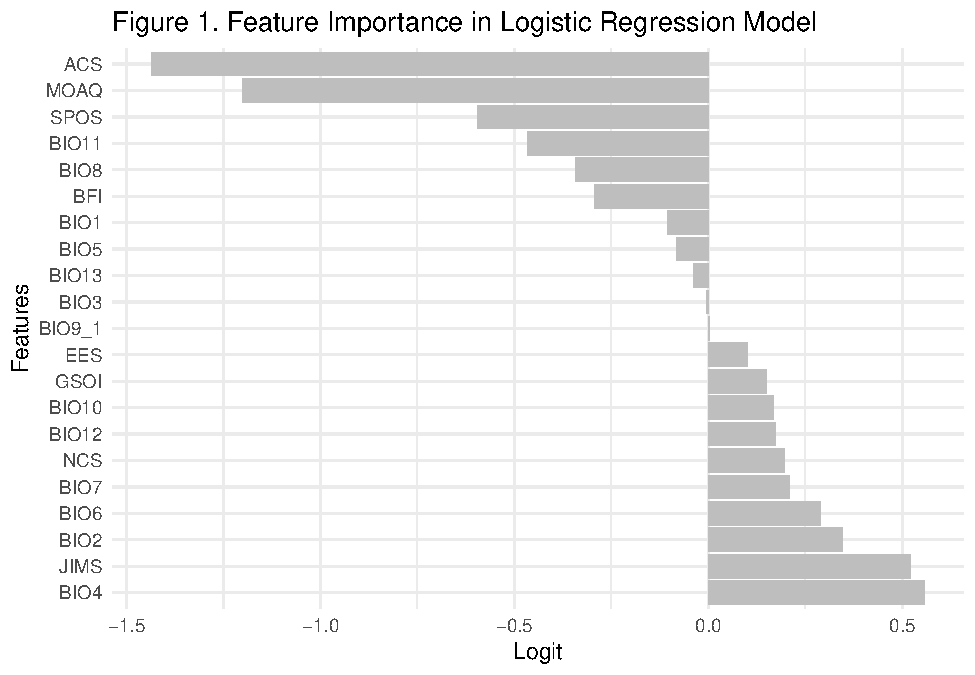
\includegraphics{dissertation_files/figure-latex/coefbg-1.pdf}
\caption{\label{fig:coefbg}Logits of the Logistic Regression}
\end{figure}

\begin{figure}
\centering
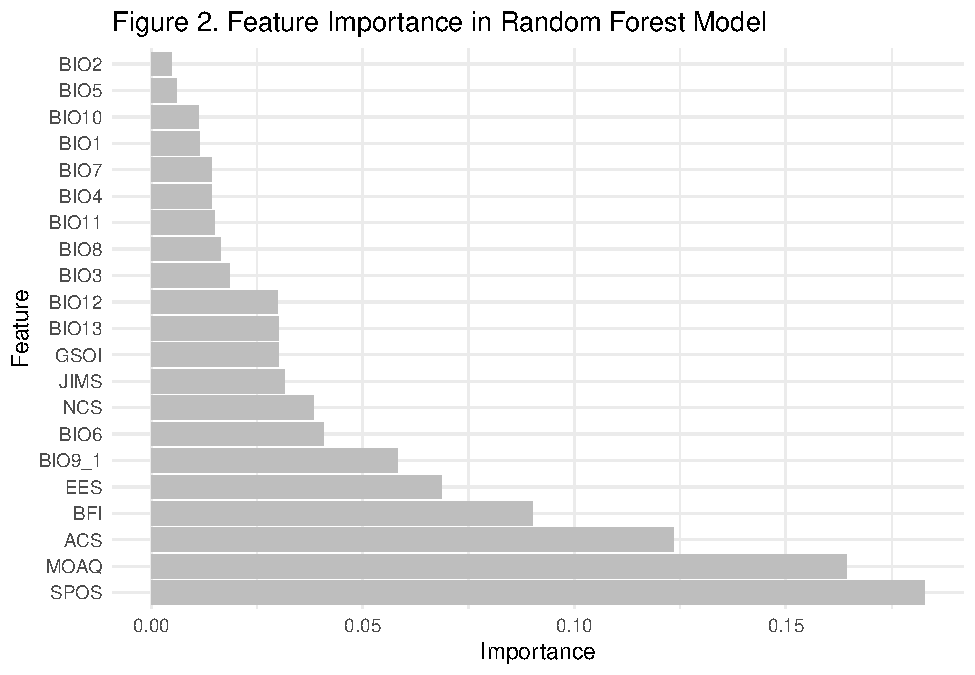
\includegraphics{dissertation_files/figure-latex/featuresbg-1.pdf}
\caption{\label{fig:featuresbg}Features Importance of a Random Forest Model}
\end{figure}

The objective of this study was to evaluate the impact of incorporating work-related psychological constructs into models trained with biodata features for predicting turnover intention. To this end, machine learning algorithms including Gradient Boosting Trees (GBT), Random Forest (RF), Neural Networks (NN) and Support Vector Machines (SVM) were employed. A logistic regression was also employed. Models were initially trained using only biodata features. Subsequently, a second series of models was developed, integrating work-related psychological constructs.

The analysis revealed a consistent enhancement in model performance upon the addition of work-related psychological constructs across all algorithms. Specifically, models incorporating work-related psychological constructs demonstrated a notable improvement in AUC-ROC scores (table \ref{tab:wrctable}) compared to those based solely on biodata features (table \ref{tab:biotable}). As can be seen in table \ref{tab:deltas}, the deltas between the AUC scores with Biodata and the AUC scores when adding WRPC to the models are on average 0.17.

The results substantiate hypothesis 3, demonstrating that models trained with both biodata features and work-related psychological constructs outperform those trained with biodata features alone. These findings underscore the value of incorporating psychological constructs into predictive models within the domain of work-related outcomes.

Additionally, as can be seen in figure \ref{fig:coefbg} and figure \ref{fig:featuresbg}, the comparative analysis of the two bar graphs, which depict feature importances derived from logistic regression and Random Forest models respectively, reveals distinct patterns in how each model values the same set of features.

In the logistic regression model, the feature ``ACS'' displayed the most significant negative coefficient, suggesting a strong inverse relationship with the target variable. In stark contrast, ``MOAQ'' and ``SPOS'' showed slightly less negative coefficients, indicating their substantial but lesser influence compared to ``ACS''. On the other hand, ``BIO4'' and ``JIMS'' had positive coefficients, albeit smaller in magnitude, pointing to their positive but modest impact on the model's predictions.

The Random Forest model presented a different hierarchy of feature importances. ``SPOS'' emerged as the most critical predictor with the highest importance score, indicating its predominant influence in the model. This was followed by ``MOAQ'' and ``ACS'', which also held significant importance but to a lesser extent than ``SPOS''. The features ``BFI'' and ``EES'', while contributing to the model, had relatively lower importance scores, suggesting their roles were not as decisive in the Random Forest model as in the logistic regression model.

\subsection{Predicting Job Satisfaction}\label{predicting-job-satisfaction}

\begin{table}[tbp]

\begin{center}
\begin{threeparttable}

\caption{\label{tab:biotable2}Biodata only model}

\begin{tabular}{ll}
\toprule
Model & \multicolumn{1}{c}{RMSE Biodata}\\
\midrule
Linear Regression & 0.58\\
XGBoost & 0.59\\
Neural Network & 0.57\\
SVM & 0.55\\
Random Forest & 0.58\\
\bottomrule
\end{tabular}

\end{threeparttable}
\end{center}

\end{table}

\begin{table}[tbp]

\begin{center}
\begin{threeparttable}

\caption{\label{tab:wrctable2}Work-related psychological constructs only model}

\begin{tabular}{ll}
\toprule
Model & \multicolumn{1}{c}{RMSE WRPC}\\
\midrule
Logistic Regression & 0.00\\
XGBoost & 0.01\\
Neural Network & 0.26\\
SVM & 0.05\\
Random Forest & 0.01\\
\bottomrule
\end{tabular}

\end{threeparttable}
\end{center}

\end{table}

\begin{table}[tbp]

\begin{center}
\begin{threeparttable}

\caption{\label{tab:deltas2}Work-related psychological constructs added to the models}

\begin{tabular}{llll}
\toprule
Model & \multicolumn{1}{c}{RMSE Biodata} & \multicolumn{1}{c}{RMSE when adding WRPC} & \multicolumn{1}{c}{Delta}\\
\midrule
Linear Regression & 0.58 & 0.45 & -0.13\\
XGBoost & 0.59 & 0.42 & -0.17\\
Neural Network & 0.57 & 0.44 & -0.13\\
SVM & 0.55 & 0.45 & -0.09\\
Random Forest & 0.58 & 0.43 & -0.15\\
\bottomrule
\end{tabular}

\end{threeparttable}
\end{center}

\end{table}

\begin{figure}
\centering
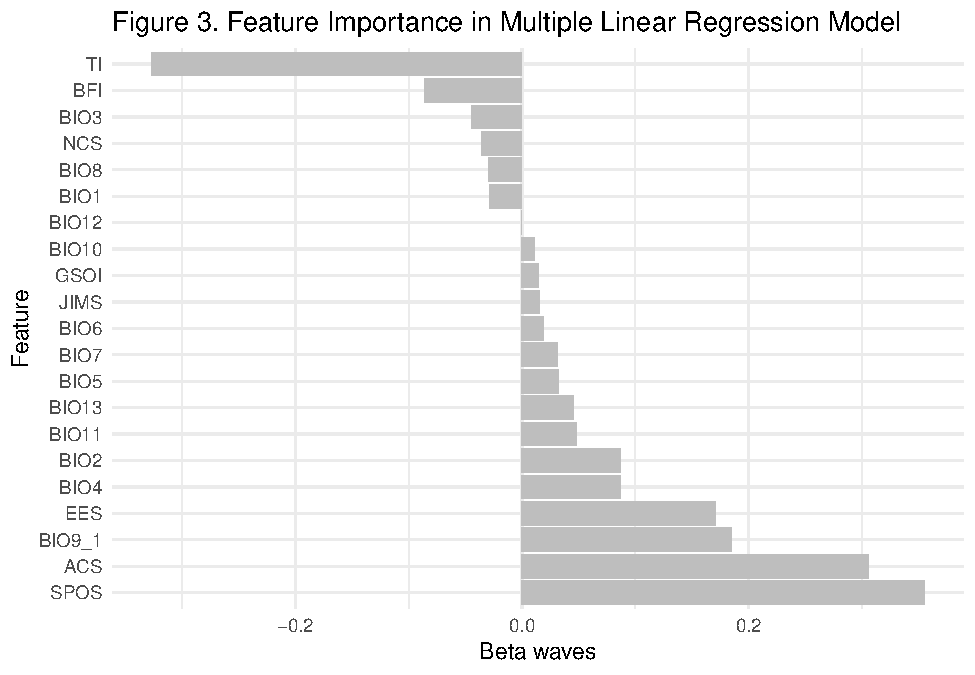
\includegraphics{dissertation_files/figure-latex/coefbg2-1.pdf}
\caption{\label{fig:coefbg2}Betas waves of the Multiple Regression}
\end{figure}

\begin{figure}
\centering
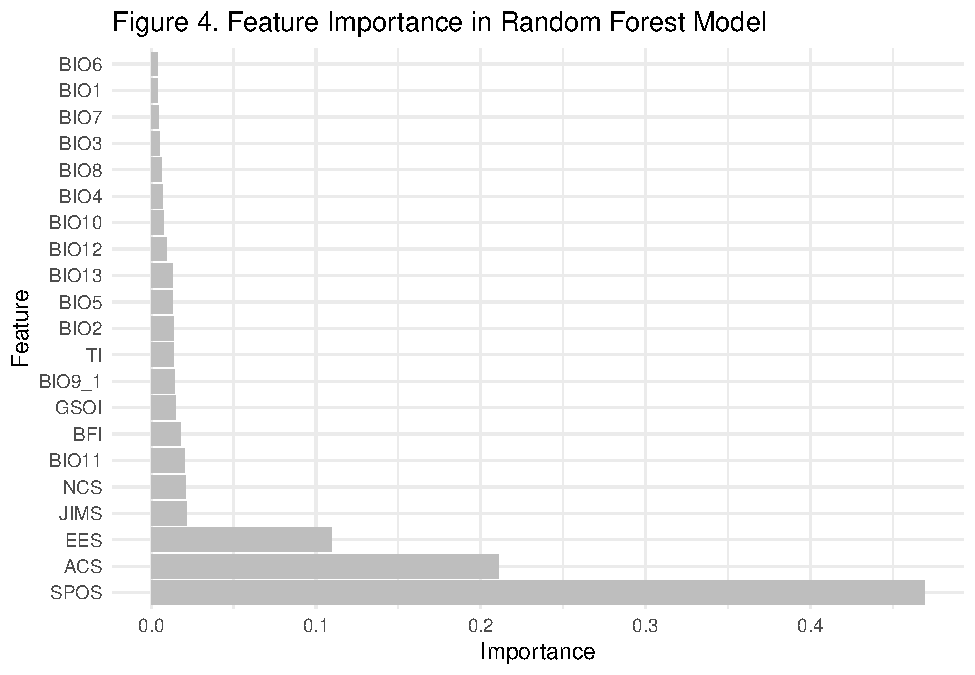
\includegraphics{dissertation_files/figure-latex/featuresbg2-1.pdf}
\caption{\label{fig:featuresbg2}Feature Importance of a Random Forest Model}
\end{figure}

The analysis revealed a consistent enhancement in model performance upon the addition of work-related psychological constructs across all algorithms. Specifically, models incorporating work-related psychological constructs demonstrated a notable improvement in RMSE scores (table \ref{tab:wrctable2}) compared to those based solely on biodata features (table \ref{tab:biotable2}). As can be seen in table \ref{tab:deltas2}, the deltas between the RMSE scores with Biodata and the RMSE scores when adding WRPC to the models are on average -0.14.

Additionally, when it comes to feature importante, both linear regression and Random Forest show similar results. As we can see in figure \ref{fig:coefbg2}, which is a bargraph showing the beta coefficients of the linear regression model, there is a balanced distribution of both positive and negative coefficients, indicating varied influences on the dependent variable. The most prominent feature in this model is ``SPOS,'' which has a positive coefficient of approximately 0.356, suggesting a strong positive relationship with the target outcome. As can be expected, ``TI'' exhibits a significant negative coefficient of -0.327. Other features like ``ACS'' and ``BIO9\_1'' also show positive influences, albeit to a lesser extent.

Conversely, figure \ref{fig:featuresbg2}, which stems from a Random Forest model, exclusively presents positive importance scores, focusing solely on the magnitude of influence rather than direction. In this model, ``SPOS'' also emerges as the most significant feature, with an importance score markedly higher at 0.470, emphasizing its critical role in model predictions. Following ``SPOS,'' ``ACS'' and ``EES'' hold substantial importance scores of 0.211 and 0.109 respectively, demonstrating their essential contributions to the model's performance.

This comparative evaluation reveals that ``SPOS'' and ``ACS'' are consistently recognized as the most influential features across both models when predicting job satisfaction.

The results substantiate hypothesis 3, demonstrating that models trained with both biodata features and work-related psychological constructs outperform those trained with biodata features alone. .

\section{Discussion}\label{discussion}

The findings of the present study do not support the hypotheses that were based on the prior research by Sanchez (2018) and Kirasich et al.~(2018). The hypotheses posited were centered around the performance of machine learning (ML) algorithms compared to regression models, with a specific focus on the effects of sample size and the number of variables on predictive accuracy. Contrary to expectations, the results from this study did not demonstrate a significant relative advantage in predictive accuracy for ML algorithms as sample size increased, nor did they confirm the hypothesized impact of the number of variables in datasets on the choice between ML and regression models.

Hypothesis 1 anticipated that as sample size increases, ML algorithms would exhibit a growing superiority over regression models in terms of predictive accuracy for turnover intentions. This hypothesis was predicated on the assertion from previous studies that ML algorithms tend to outperform regression models in larger datasets due to their ability to handle high-dimensional data and complex model interactions (Sanchez, 2018; Kirasich et al., 2018). However, the current study's findings suggest that the predictive accuracy of ML algorithms does not significantly outpace that of regression models as sample sizes increase. This discrepancy might be attributed to several factors including the nature of the data, the specific algorithms employed, or the methodologies used in the current study compared to those in the cited research.

Hypothesis 2 was based on the observation that ML algorithms perform less effectively in terms of predictive accuracy when the number of predictors in a dataset is limited, particularly when the events per variable (EPV) are below 200. This hypothesis did find support in the current study's results, suggesting that the number of variables may be a determinant factor in the efficacy of ML algorithms compared to regression models. This finding is consistent with the conclusions drawn by Sanchez (2018), where it was noted that regression models held a consistent or improved predictive accuracy under similar conditions. It is possible that advancements in ML techniques or variations in data preprocessing and feature engineering might have influenced the outcomes observed in the current study.

The absence of expected findings in study 1 calls for a careful consideration of the conditions under which previous research asserted the superiority of ML over traditional statistical methods. It may be necessary to conduct further investigations into how specific characteristics of data, such as the structure and quality of the dataset, influence the performance of different analytical approaches. Additionally, the replication of this study across various contexts and with different types of data might help in understanding the nuanced dynamics between ML algorithms and regression models.

In conclusion, while the current study does not support the hypothesized advantages of ML algorithms over regression models with respect to sample size, these results contribute to the ongoing dialogue and exploration into the most effective analytical techniques in predictive modeling. Future research should continue to explore these dynamics, perhaps focusing on different types of outcomes, varying conditions of data complexity, and the integration of novel machine learning methodologies.

As Richard Landers said in an interview with SIOP, ``Let's blend I-O psychology's tried-and-true practices where we know what we're measuring and we're very confident in the kinds of recommendations we're giving, and let's figure out where the intersections are with some of the new stuff coming out, to figure out what is truly new and useful and what is just a faddish waste of time.'' (Landers, 2019).
Many of the new technological developments in the fields of data science and computers science are not backed by the expertise that I/O psychology has been developing over the years, yet they appear more attractive for many HR practices.
It is important that we blend with these communities and contribute with our knowledge, otherwise, as Landers puts it, ``they're going to run away with the farm,'' (Landers, 2019).
A way in which the field of I/O psychology could contribute in the development of machine learning solutions for HR practices would be to build algorithms that use antecedents of job performance commonly studied by I/O psychology researchers as input variables.
These could be variables such as organizational commitment, organizational engagement, organizational identification, perceived organizational support, perceived organizational justice, etc.
Showing evidence of incremental predictive accuracy over algorithms built with other types of input would encourage better practices.
Although machine learning algorithms have the advantage that they can learn from the data and look at associations between variables that would need to be specified if a regression technique was used instead, they are also very data hungry.
This makes them viable for fortune 500 companies, for instance, but in most contexts there's the possibility that regression methods will produce the same predictive accuracy (or perhaps even better) without having to sacrifice parsimony and sparsity.
It is also important to be selective on the variables that are being fed to the algorithms, since using all and any data that gives good predictive performance could lead to the aforementioned GIGO issue (``garbage in, garbage out'').
Input may be subjective (and/or biased), particularly if there are IVs such as ``previous performance''.
This GIGO issue might be exacerbated by peoples' awe and wonder of ML.
Using variables supported by previous research would be best practice in building these ML solutions.

\newpage

\section{References}\label{references}

\phantomsection\label{refs}
\begin{CSLReferences}{1}{0}
\bibitem[\citeproctext]{ref-alpaydin2020introduction}
Alpaydin, E. (2020). \emph{Introduction to machine learning}. MIT press.

\bibitem[\citeproctext]{ref-alzate2022predictions}
Alzate Vanegas, J. M., Wine, W., \& Drasgow, F. (2022). Predictions of attrition among US marine corps: Comparison of four predictive methods. \emph{Military Psychology}, \emph{34}(2), 147--166.

\bibitem[\citeproctext]{ref-barandela2003new}
Barandela, R., Valdovinos, R. M., \& Sánchez, J. S. (2003). New applications of ensembles of classifiers. \emph{Pattern Analysis \& Applications}, \emph{6}, 245--256.

\bibitem[\citeproctext]{ref-beam2018big}
Beam, A. L., \& Kohane, I. S. (2018). Big data and machine learning in health care. \emph{Jama}, \emph{319}(13), 1317--1318.

\bibitem[\citeproctext]{ref-biswas2020prediction}
Biswas, S., Fernandez Castellanos, D., \& Zaiser, M. (2020). Prediction of creep failure time using machine learning. \emph{Scientific Reports}, \emph{10}(1), 16910.

\bibitem[\citeproctext]{ref-boulesteix2014machine}
Boulesteix, A.-L., \& Schmid, M. (2014). Machine learning versus statistical modeling. \emph{Biometrical Journal}, \emph{56}(4), 588--593.

\bibitem[\citeproctext]{ref-breiman2001random}
Breiman, L. (2001a). Random forests. \emph{Machine Learning}, \emph{45}, 5--32.

\bibitem[\citeproctext]{ref-breiman2001statistical}
Breiman, L. (2001b). Statistical modeling: The two cultures (with comments and a rejoinder by the author). \emph{Statistical Science}, \emph{16}(3), 199--231.

\bibitem[\citeproctext]{ref-chipman2010bart}
Chipman, H. A., George, E. I., \& McCulloch, R. E. (2010). \emph{BART: Bayesian additive regression trees}.

\bibitem[\citeproctext]{ref-cho2012turnover}
Cho, Y. J., \& Lewis, G. B. (2012). Turnover intention and turnover behavior: Implications for retaining federal employees. \emph{Review of Public Personnel Administration}, \emph{32}(1), 4--23.

\bibitem[\citeproctext]{ref-choi2011organizational}
Choi, S. (2011). Organizational justice and employee work attitudes: The federal case. \emph{The American Review of Public Administration}, \emph{41}(2), 185--204.

\bibitem[\citeproctext]{ref-cohen2016does}
Cohen, G., Blake, R. S., \& Goodman, D. (2016). Does turnover intention matter? Evaluating the usefulness of turnover intention rate as a predictor of actual turnover rate. \emph{Review of Public Personnel Administration}, \emph{36}(3), 240--263.

\bibitem[\citeproctext]{ref-collins2014external}
Collins, G. S., Groot, J. A. de, Dutton, S., Omar, O., Shanyinde, M., Tajar, A., Voysey, M., Wharton, R., Yu, L.-M., Moons, K. G., et al. (2014). External validation of multivariable prediction models: A systematic review of methodological conduct and reporting. \emph{BMC Medical Research Methodology}, \emph{14}(1), 1--11.

\bibitem[\citeproctext]{ref-cox1972regression}
Cox, D. R. (1972). Regression models and life-tables. \emph{Journal of the Royal Statistical Society: Series B (Methodological)}, \emph{34}(2), 187--202.

\bibitem[\citeproctext]{ref-craninx2008artificial}
Craninx, M., Fievez, V., Vlaeminck, B., \& De Baets, B. (2008). Artificial neural network models of the rumen fermentation pattern in dairy cattle. \emph{Computers and Electronics in Agriculture}, \emph{60}(2), 226--238.

\bibitem[\citeproctext]{ref-cristianini2002support}
Cristianini, N., \& Scholkopf, B. (2002). Support vector machines and kernel methods: The new generation of learning machines. \emph{Ai Magazine}, \emph{23}(3), 31--31.

\bibitem[\citeproctext]{ref-davis2006relationship}
Davis, J., \& Goadrich, M. (2006). The relationship between precision-recall and ROC curves. \emph{Proceedings of the 23rd International Conference on Machine Learning}, 233--240.

\bibitem[\citeproctext]{ref-deo2016learning}
Deo, R. C., \& Nallamothu, B. K. (2016). Learning about machine learning: The promise and pitfalls of big data and the electronic health record. In \emph{Circulation: Cardiovascular Quality and Outcomes} (No. 6; Vol. 9, pp. 618--620). Am Heart Assoc.

\bibitem[\citeproctext]{ref-dietterich2000ensemble}
Dietterich, T. G. (2000). Ensemble methods in machine learning. \emph{International Workshop on Multiple Classifier Systems}, 1--15.

\bibitem[\citeproctext]{ref-douglass2020book}
Douglass, M. J. (2020). \emph{Book review: Hands-on machine learning with scikit-learn, keras, and tensorflow, by aur{é}lien g{é}ron: O'reilly media, 2019, 600 pp., ISBN: 978-1-492-03264-9}. Springer.

\bibitem[\citeproctext]{ref-ertas2015turnover}
Ertas, N. (2015). Turnover intentions and work motivations of millennial employees in federal service. \emph{Public Personnel Management}, \emph{44}(3), 401--423.

\bibitem[\citeproctext]{ref-fallucchi2020predicting}
Fallucchi, F., Coladangelo, M., Giuliano, R., \& William De Luca, E. (2020). Predicting employee attrition using machine learning techniques. \emph{Computers}, \emph{9}(4), 86.

\bibitem[\citeproctext]{ref-franzen2022developing}
Franzen, P., Arens, A. K., Greiff, S., Westhuizen, L. van der, Fischbach, A., Wollschläger, R., \& Niepel, C. (2022). Developing and validating a short-form questionnaire for the assessment of seven facets of conscientiousness in large-scale assessments. \emph{Journal of Personality Assessment}, \emph{104}(6), 759--773.

\bibitem[\citeproctext]{ref-froud2021relative}
Froud, R., Hansen, S. H., Ruud, H. K., Foss, J., Ferguson, L., \& Fredriksen, P. M. (2021). Relative performance of machine learning and linear regression in predicting quality of life and academic performance of school children in norway: Data analysis of a quasi-experimental study. \emph{Journal of Medical Internet Research}, \emph{23}(7), e22021.

\bibitem[\citeproctext]{ref-griffeth2000meta}
Griffeth, R. W., Hom, P. W., \& Gaertner, S. (2000). A meta-analysis of antecedents and correlates of employee turnover: Update, moderator tests, and research implications for the next millennium. \emph{Journal of Management}, \emph{26}(3), 463--488.

\bibitem[\citeproctext]{ref-guyon2003introduction}
Guyon, I., \& Elisseeff, A. (2003). An introduction to variable and feature selection. \emph{Journal of Machine Learning Research}, \emph{3}(Mar), 1157--1182.

\bibitem[\citeproctext]{ref-hastie2009elements}
Hastie, T., Tibshirani, R., Friedman, J. H., \& Friedman, J. H. (2009). \emph{The elements of statistical learning: Data mining, inference, and prediction} (Vol. 2). Springer.

\bibitem[\citeproctext]{ref-he2009learning}
He, H., \& Garcia, E. A. (2009). Learning from imbalanced data. \emph{IEEE Transactions on Knowledge and Data Engineering}, \emph{21}(9), 1263--1284.

\bibitem[\citeproctext]{ref-hom2012reviewing}
Hom, P. W., Mitchell, T. R., Lee, T. W., \& Griffeth, R. W. (2012). Reviewing employee turnover: Focusing on proximal withdrawal states and an expanded criterion. \emph{Psychological Bulletin}, \emph{138}(5), 831.

\bibitem[\citeproctext]{ref-hom2009explaining}
Hom, P. W., Tsui, A. S., Wu, J. B., Lee, T. W., Zhang, A. Y., Fu, P. P., \& Li, L. (2009). Explaining employment relationships with social exchange and job embeddedness. \emph{Journal of Applied Psychology}, \emph{94}(2), 277.

\bibitem[\citeproctext]{ref-hosmer2013applied}
Hosmer Jr, D. W., Lemeshow, S., \& Sturdivant, R. X. (2013). \emph{Applied logistic regression} (Vol. 398). John Wiley \& Sons.

\bibitem[\citeproctext]{ref-kermany2018identifying}
Kermany, D. S., Goldbaum, M., Cai, W., Valentim, C. C., Liang, H., Baxter, S. L., McKeown, A., Yang, G., Wu, X., Yan, F., et al. (2018). Identifying medical diagnoses and treatable diseases by image-based deep learning. \emph{Cell}, \emph{172}(5), 1122--1131.

\bibitem[\citeproctext]{ref-kim2017employee}
Kim, S. Y., \& Fernandez, S. (2017). Employee empowerment and turnover intention in the US federal bureaucracy. \emph{The American Review of Public Administration}, \emph{47}(1), 4--22.

\bibitem[\citeproctext]{ref-kirasich2018random}
Kirasich, K., Smith, T., \& Sadler, B. (2018). Random forest vs logistic regression: Binary classification for heterogeneous datasets. \emph{SMU Data Science Review}, \emph{1}(3), 9.

\bibitem[\citeproctext]{ref-kubat1997addressing}
Kubat, M., Matwin, S., et al. (1997). Addressing the curse of imbalanced training sets: One-sided selection. \emph{Icml}, \emph{97}, 179.

\bibitem[\citeproctext]{ref-lawler1979michigan}
Lawler, E., Cammann, C., Nadler, D., \& Jenkins, D. (1979). Michigan organizational assessment questionnaire. \emph{Journal of Vocational Behavior}.

\bibitem[\citeproctext]{ref-lee2021overlooked}
Lee, G. R., Fernandez, S., \& Lee, S. (2021). An overlooked cost of contracting out: Evidence from employee turnover intention in US federal agencies. \emph{Public Personnel Management}, \emph{50}(3), 381--407.

\bibitem[\citeproctext]{ref-liss2015loving}
Liss-Levinson, R., Bharthapudi, K., Leider, J. P., \& Sellers, K. (2015). Loving and leaving public health: Predictors of intentions to quit among state health agency workers. \emph{Journal of Public Health Management and Practice}, \emph{21}(Suppl 6), S91.

\bibitem[\citeproctext]{ref-luu2020machine}
Luu, B. C., Wright, A. L., Haeberle, H. S., Karnuta, J. M., Schickendantz, M. S., Makhni, E. C., Nwachukwu, B. U., Williams III, R. J., \& Ramkumar, P. N. (2020). Machine learning outperforms logistic regression analysis to predict next-season NHL player injury: An analysis of 2322 players from 2007 to 2017. \emph{Orthopaedic Journal of Sports Medicine}, \emph{8}(9), 2325967120953404.

\bibitem[\citeproctext]{ref-macijauskieneartificial}
Macijauskien, I., \& Stankevi, ivil. (2021). Artificial intelligence solution in human resources management: Case study of chatbot's implication. \emph{STRATEGICA}, 517.

\bibitem[\citeproctext]{ref-maertz2007effects}
Maertz Jr, C. P., Griffeth, R. W., Campbell, N. S., \& Allen, D. G. (2007). The effects of perceived organizational support and perceived supervisor support on employee turnover. \emph{Journal of Organizational Behavior: The International Journal of Industrial, Occupational and Organizational Psychology and Behavior}, \emph{28}(8), 1059--1075.

\bibitem[\citeproctext]{ref-mahesh2020machine}
Mahesh, B. (2020). Machine learning algorithms-a review. \emph{International Journal of Science and Research (IJSR).{[}Internet{]}}, \emph{9}(1), 381--386.

\bibitem[\citeproctext]{ref-marsland2011machine}
Marsland, S. (2011). \emph{Machine learning: An algorithmic perspective}. Chapman; Hall/CRC.

\bibitem[\citeproctext]{ref-meyer1991three}
Meyer, J. P., \& Allen, N. J. (1991). A three-component conceptualization of organizational commitment. \emph{Human Resource Management Review}, \emph{1}(1), 61--89.

\bibitem[\citeproctext]{ref-meyer2004employee}
Meyer, J. P., Becker, T. E., \& Vandenberghe, C. (2004). Employee commitment and motivation: A conceptual analysis and integrative model. \emph{Journal of Applied Psychology}, \emph{89}(6), 991.

\bibitem[\citeproctext]{ref-miller2016finding}
Miller, P. J., Lubke, G. H., McArtor, D. B., \& Bergeman, C. (2016). Finding structure in data using multivariate tree boosting. \emph{Psychological Methods}, \emph{21}(4), 583.

\bibitem[\citeproctext]{ref-mitchell1997machine}
Mitchell, T. M. (1997). \emph{Machine learning}.

\bibitem[\citeproctext]{ref-mitchell2001people}
Mitchell, T. R., Holtom, B. C., Lee, T. W., Sablynski, C. J., \& Erez, M. (2001). Why people stay: Using job embeddedness to predict voluntary turnover. \emph{Academy of Management Journal}, \emph{44}(6), 1102--1121.

\bibitem[\citeproctext]{ref-mobley1979review}
Mobley, W. H., Griffeth, R. W., Hand, H. H., \& Meglino, B. M. (1979). Review and conceptual analysis of the employee turnover process. \emph{Psychological Bulletin}, \emph{86}(3), 493.

\bibitem[\citeproctext]{ref-myers2013research}
Myers, J. L., Well, A. D., \& Lorch Jr, R. F. (2013). \emph{Research design and statistical analysis}. Routledge.

\bibitem[\citeproctext]{ref-niculescu2005predicting}
Niculescu-Mizil, A., \& Caruana, R. (2005). \emph{Predicting good probabilities with supervised learning}. 625--632.

\bibitem[\citeproctext]{ref-pitts2011so}
Pitts, D., Marvel, J., \& Fernandez, S. (2011). So hard to say goodbye? Turnover intention among US federal employees. \emph{Public Administration Review}, \emph{71}(5), 751--760.

\bibitem[\citeproctext]{ref-van2014modern}
Ploeg, T. van der, Austin, P. C., \& Steyerberg, E. W. (2014). Modern modelling techniques are data hungry: A simulation study for predicting dichotomous endpoints. \emph{BMC Medical Research Methodology}, \emph{14}(1), 1--13.

\bibitem[\citeproctext]{ref-rkab2019recruitment}
Rąb-Kettler, K., \& Lehnervp, B. (2019). Recruitment in the times of machine learning. \emph{Management Systems in Production Engineering}.

\bibitem[\citeproctext]{ref-raji2019actionable}
Raji, I. D., \& Buolamwini, J. (2019). Actionable auditing: Investigating the impact of publicly naming biased performance results of commercial ai products. \emph{Proceedings of the 2019 AAAI/ACM Conference on AI, Ethics, and Society}, 429--435.

\bibitem[\citeproctext]{ref-reeve2001refining}
Reeve, C. L., \& Smith, C. S. (2001). Refining lodahl and kejner's job involvement scale with a convergent evidence approach: Applying multiple methods to multiple samples. \emph{Organizational Research Methods}, \emph{4}(2), 91--111.

\bibitem[\citeproctext]{ref-sanchez2018big}
Sanchez-Pinto, L. N., Luo, Y., \& Churpek, M. M. (2018). Big data and data science in critical care. \emph{Chest}, \emph{154}(5), 1239--1248.

\bibitem[\citeproctext]{ref-sanchez2018comparison}
Sanchez-Pinto, L. N., Venable, L. R., Fahrenbach, J., \& Churpek, M. M. (2018). Comparison of variable selection methods for clinical predictive modeling. \emph{International Journal of Medical Informatics}, \emph{116}, 10--17.

\bibitem[\citeproctext]{ref-schaufeli2017ultra}
Schaufeli, W. B., Shimazu, A., Hakanen, J., Salanova, M., \& De Witte, H. (2017). An ultra-short measure for work engagement. \emph{European Journal of Psychological Assessment}.

\bibitem[\citeproctext]{ref-schoenfeldt1999dust}
Schoenfeldt, L. F. (1999). From dust bowl empiricism to rational constructs in biographical data. \emph{Human Resource Management Review}, \emph{9}(2), 147--167.

\bibitem[\citeproctext]{ref-seashore1983assessing}
Seashore, S. E., Lawler III, E. E., Mirvis, P. H., \& Cammann, C. E. (1983). \emph{Assessing organizational change: A guide to methods, measures, and practices.} John Wiley \& Sons Inc.

\bibitem[\citeproctext]{ref-shamir2004single}
Shamir, B., \& Kark, R. (2004). A single-item graphic scale for the measurement of organizational identification. \emph{Journal of Occupational and Organizational Psychology}, \emph{77}(1), 115--123.

\bibitem[\citeproctext]{ref-shore1991construct}
Shore, L. M., \& Tetrick, L. E. (1991). A construct validity study of the survey of perceived organizational support. \emph{Journal of Applied Psychology}, \emph{76}(5), 637.

\bibitem[\citeproctext]{ref-smith2005achieving}
Smith, I. (2005). Achieving readiness for organisational change. \emph{Library Management}, \emph{26}(6/7), 408--412.

\bibitem[\citeproctext]{ref-tambe2019artificial}
Tambe, P., Cappelli, P., \& Yakubovich, V. (2019). Artificial intelligence in human resources management: Challenges and a path forward. \emph{California Management Review}, \emph{61}(4), 15--42.

\bibitem[\citeproctext]{ref-varoquaux2018cross}
Varoquaux, G. (2018). Cross-validation failure: Small sample sizes lead to large error bars. \emph{Neuroimage}, \emph{180}, 68--77.

\bibitem[\citeproctext]{ref-vijayakumar2019replicability}
Vijayakumar, R., \& Cheung, M. W.-L. (2019). Replicability of machine learning models in the social sciences. \emph{Zeitschrift F{ü}r Psychologie}.

\bibitem[\citeproctext]{ref-xu2020deep}
Xu, X., Jiang, X., Ma, C., Du, P., Li, X., Lv, S., Yu, L., Ni, Q., Chen, Y., Su, J., et al. (2020). A deep learning system to screen novel coronavirus disease 2019 pneumonia. \emph{Engineering}, \emph{6}(10), 1122--1129.

\bibitem[\citeproctext]{ref-zou2018ai}
Zou, J., \& Schiebinger, L. (2018). \emph{AI can be sexist and racist---it's time to make it fair}. Nature Publishing Group UK London.

\end{CSLReferences}

\newpage

\appendix

\section{2}\label{aptables}


\clearpage
\renewcommand{\listfigurename}{Figure captions}

\clearpage
\renewcommand{\listtablename}{Table captions}


\end{document}
